\documentclass{beamer}

\input{preamble.tex}
\usepackage{breqn} % Breaks lines

\usepackage{amsmath}
\usepackage{mathtools}

\usepackage{pdfpages} % \includepdf

\usepackage{listings} % R code
\usepackage{verbatim} % verbatim

% Video stuff
\usepackage{media9}

% packages for bibs and cites
\usepackage{natbib}
\usepackage{har2nat}
\newcommand{\possessivecite}[1]{\citeauthor{#1}'s \citeyearpar{#1}}
\usepackage{breakcites}
\usepackage{alltt}

% Setup math operators
\DeclareMathOperator{\E}{E} \DeclareMathOperator{\tr}{tr} \DeclareMathOperator{\se}{se} \DeclareMathOperator{\I}{I} \DeclareMathOperator{\sign}{sign} \DeclareMathOperator{\supp}{supp} \DeclareMathOperator{\plim}{plim}
\DeclareMathOperator*{\dlim}{\mathnormal{d}\mkern2mu-lim}
\newcommand\independent{\protect\mathpalette{\protect\independenT}{\perp}}
   \def\independenT#1#2{\mathrel{\rlap{$#1#2$}\mkern2mu{#1#2}}}
\newcommand*\colvec[1]{\begin{pmatrix}#1\end{pmatrix}}

\newcommand{\myurlshort}[2]{\href{#1}{\textcolor{gray}{\textsf{#2}}}}


\begin{document}

\imageframe{./lecture_includes/mixtape_did_cover.png}


% ---- Content ----

\section{Introduction}

\subsection{Managing expectations}


\begin{frame}{Introduction}

\begin{itemize}
\item Thank you coming to Mixtape Sessions' Causal Inference 2 workshop on difference-in-differences!  
\item Scott Cunningham, Ben H. Williams Professor of Economics at Baylor University in Texas USA
\item Kyle Butts, UC-Boulder (PhD), University of Arkansas (Assistant Professor) in USA
\item 9:00am to 5:00pm CST, 15 min breaks every hour, 1 hour lunch at 12:00
\item Lecture, discussion, exercises, application with "live coding" exercises
\end{itemize}

\end{frame}


\begin{frame}{What my pedagogy is like}

\begin{itemize}
\item High energy, eclectic approach to teaching
\item Move between the econometrics, history of thought, videos, applications, code, spreadsheets, exercises
\item Workshop is intended to take someone from knowing nothing about difference-in-differences to nearly the cutting edge
\item Ask questions at any point; I'll do my best to answer them
\end{itemize}

\end{frame}


\begin{frame}{Class goals}
Pedagogical goal is to break down the procedures into plain English, rebuilding it into something you can and want to use, but also:

  \begin{enumerate}
    \item \textbf{Confidence}: You will feel like you have a good enough understanding of diff-in-diff and synthetic control, both in its basics and some more contemporary issues, so that by the end of the week it a very intuitive, friendly, and useful tool
    \item \textbf{Comprehension}: You will have learned a lot both conceptually and in the specifics, particularly with regards to issues around identification and estimation in the diff-in-diff and synth context
    \item \textbf{Competency}: You will have more knowledge of programming syntax in Stata and R so that later you can apply this in your own work
  \end{enumerate}

\end{frame}



\begin{frame}{Day 1 outline}

Basics of difference-in-differences (Beginners but also my own personal take on this)
	\begin{itemize}
	\item Potential outcomes review and the ATT parameter
	\item DiD equation (``four averages and three differences''), parallel trends and estimation with OLS specification and inference
	\item Simple exercises illustrating potential outcomes, parameters, diff-in-diff and parallel trends
	\item Five step evidence of difference-in-differences
	\item Event study
	\item Triple differences (design) vs Falsifications (not a design)
	\item \textbf{Homework!}
	\end{itemize}

\end{frame}


\begin{frame}{Day 2 outline}

Violations of parallel trends
	\begin{itemize}
	\item \textbf{Review Homework!}
	\item Repeated cross sections and compositional change
	\item Incorporating covariates
		\begin{itemize}
		\item Heckman, Ichimura and Todd (1997)
		\item Abadie (2005)
		\item Sant’Anna and Zhao (2020)
		\item Twoway fixed effects with time varying controls	
		\end{itemize}
	\item Lalonde coding exercise
	\item Hands-on example
	\end{itemize}

\end{frame}

\begin{frame}{Day 3 outline}

Pathologies of and Solutions to Twoway Fixed Effects with Differential Timing
	\begin{itemize}
	\item Panel fixed effects and strict exogeneity (Cunningham 2021) 
	\item ``Old school'' example using Cheng and Hoekstra (2013) “Castle Doctrine” paper
	\item Bacon decomposition (Goodman-Bacon 2021)
	\item Aggregate ATT(g,t) method (Callaway and Sant’Anna 2021)
	\item Simple illustrations in simulations
	\item Walk through R shiny app
	\end{itemize}

\end{frame}


\begin{frame}{Day 4 outline}

Event studies and staggered, Imputation estimators

\begin{itemize}
\item Decomposition event study leads and lags under staggered adoption (Sun and Abraham 2021)
\item Imputation estimators
		\begin{itemize}
		\item Borusyak, et al. (2023) “robust efficient imputation estimator”
		\item Gardner, et al. (2023) two stage difference in differences
		\end{itemize}
\item Discussion of two contemporary papers using these methods and the presentation of results
\item Simple simulation with Cunningham
\item Continuous treatment difference-in-differences (Callaway, Goodman-Bacon and Sant'Anna 2024)
\end{itemize}

\end{frame}




\subsection{Origins of diff-in-diff in public health}



\begin{frame}{Common view of diff-in-diff}

\begin{figure}
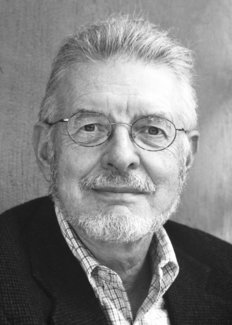
\includegraphics[scale=1.5]{./lecture_includes/mcfadden.jpg}
\end{figure}

\begin{quote}
``A good way to do econometrics is to look for good natural experiments and use statistical methods that can tidy up the confounding factors that nature has not controlled for us.'' -- Daniel McFadden (Nobel Laureate 2002)
\end{quote}


\end{frame}



\begin{frame}{What is difference-in-differences (DiD)}

\begin{itemize}
\item DiD is when a group of units are assigned some treatment and then compared to a group of units that weren't before and after
\item One of the most widely used quasi-experimental methods in economics and increasingly in industry
\item Predates the randomized experiment by 80 years, but uses basic experimental ideas about treatment and control groups (just not randomized)
\item Uses panel or repeated cross section datasets, binary treatments usually, and often covariates
\item We'll do a quick run through the social history of diff-in-diff to set the stage for our workshop this week
\end{itemize}
\end{frame}








\begin{frame}{Ignaz Semmelweis and washing hands}

\begin{itemize}
\item Early 1820s, Vienna passed legislation requiring that if a pregnant women giving birth went to a public hospital (free care), then depending on the day of week and time of day, she would be routed to either the midwife wing or the physician wing (most likely resulting in random assignment)
\item But by the 1840s, Ignaz Semmelweis noticed that pregnant women died after delivery in the (male) wing at a rate of 13-18\%, but only 3\% in the (female) midwife wing -- cause was puerperal or “childbed” fever
\item Somehow this was also we known -- women would give birth in the street rather than go to the physician if they were unlucky enough to have their water break on the wrong day and time
\end{itemize}

\end{frame}

\begin{frame}{Ignaz Semmelweis and washing hands}

\begin{itemize}
\item Ignaz Semmelweis conjectures after a lot of observation that the cause is the teaching faculty teaching anatomy using cadavers and then delivering babies \emph{without washing hands}
\item New training happens to one but not the other and Semmelweis thinks the mortality is caused by working with cadavers
\item Convinced the hospital to have physicians wash their hands in chlorine but not the midwives, creating a type of difference-in-differences design 
\end{itemize}

\end{frame}

\begin{frame}{Semmelweis diff-in-diff evidence}

	\begin{figure}
	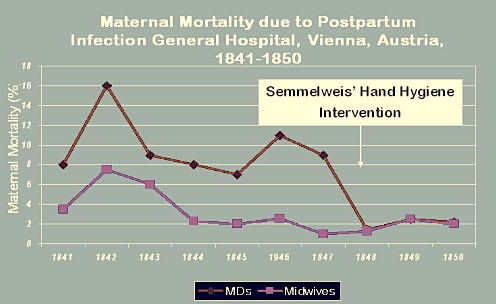
\includegraphics[scale=0.5]{./lecture_includes/semmelweis_graph.jpg}
	\end{figure}


\end{frame}

\begin{frame}{Evidence Rejected}

\begin{itemize}

\item Diff-in-diff evidence was rejected by Semmelweis' superiors claiming it was the hospital's new ventilation system
\item Dominant theory of disease spread was caused by "odors" or miasma or "humors"
\item Semmelweis began showing signs of irritability, perhaps onset of dementia, became publicly abusive, was committed to a mental hospital and within two weeks died from wounds he received while in residence
\item Despite the strength of evidence, difference-in-differences was rejected -- a theme we will see continue

\end{itemize}

\end{frame}






\begin{frame}{John Snow and cholera}

\begin{itemize}
\item Three major waves of cholera in the early to mid 1800s in London, largely thought to be spread by miasma (``dirty air'')
\item John Snow believed cholera was spread through the Thames water supply through an invisible creature that entered the body through food and drink, caused the body to expel water, placing the creature back in the Thames and causing epidemic waves
\item London passes ordinance requiring water utility companies to move inlet pipe further up the Thames, above the city center, but not everyone complies
\item Natural experiment: Lambeth water company moves its pipe between 1849 and 1854; Southwark and Vauxhall water company delayed
\end{itemize}

\end{frame}


\begin{frame}

	\begin{figure}
	\caption{Two water utility companies in London 1854}
	\includegraphics[scale=0.225]{./lecture_includes/lambeth.png}
	\end{figure}


\end{frame}



\begin{frame}{Difference-in-differences}

\begin{table}\centering
\scriptsize
		\caption{Lambeth and Southwark and Vauxhall, 1849 and 1854}
		\begin{center}
		\begin{tabular}{lll|lc}
		\toprule
		\multicolumn{1}{l}{\textbf{Companies}}&
		\multicolumn{1}{c}{\textbf{Time}}&
		\multicolumn{1}{c}{\textbf{Outcome}}&
		\multicolumn{1}{c}{$D_1$}&
		\multicolumn{1}{c}{$D_2$}\\
		\midrule
		Lambeth & Before & $Y=L$ \\
		& After & $Y=L + L_t + D$ & $\textcolor{red}{L_t}+D$\\
		\midrule
		& & & & $D + (\textcolor{red}{L_t}- SV_t)$ \\
		\midrule
		Southwark and Vauxhall & Before & $Y=SV$ \\
		& After & $Y=SV + SV_t$ & $SV_t$\\
		\bottomrule
		\end{tabular}
		\end{center}
	\end{table}

\begin{eqnarray*}
\widehat{\delta}_{did} = D + (\textcolor{red}{L_t}- SV_t)
\end{eqnarray*}This method yields an unbiased estimate of D if $\textcolor{red}{L_t} = SV_t$, but note that $\textcolor{red}{L_t}$ is a counterfactual trend and therefore not known

\end{frame}






\subsection{Three waves of Difference-in-Differences in Economics}

\begin{frame}{Growing popularity in economics}

	\begin{figure}
	\caption{Currie, et al. (2020)}
	\includegraphics[scale=0.25]{./lecture_includes/currie_did.png}
	\end{figure}

\bigskip

\footnotesize

With some exception (e.g., Heckman, Ichimura and Todd 1997; Abadie 2005; Bertrand, Duflo and Mullainthan 2004), econometricians had not given it much notice

\end{frame}



\begin{frame}{First Wave of Diff-in-Diff}

\begin{itemize}
\item Difference-in-differences evolved in three waves from 1983 to present in economics
\item First wave lasts from 1983 to 2011; second wave from 2011 to 2018; third wave from 2018 to present
\item Initially, mostly used by labor economists throughout the 1990s in the ``program evaluation'' area but spreads with the spread of causal inference 
\item No potential outcomes notation, no mention of parallel trends, no event studies -- only Ashenfelter's Dip, evidence of time varying selection bias

\end{itemize}

\end{frame}


\begin{frame}{Ashenfelter and Card coin the phrase difference-in-differences}

	\begin{figure}
	\caption{Ashenfelter and Card (1983)}
	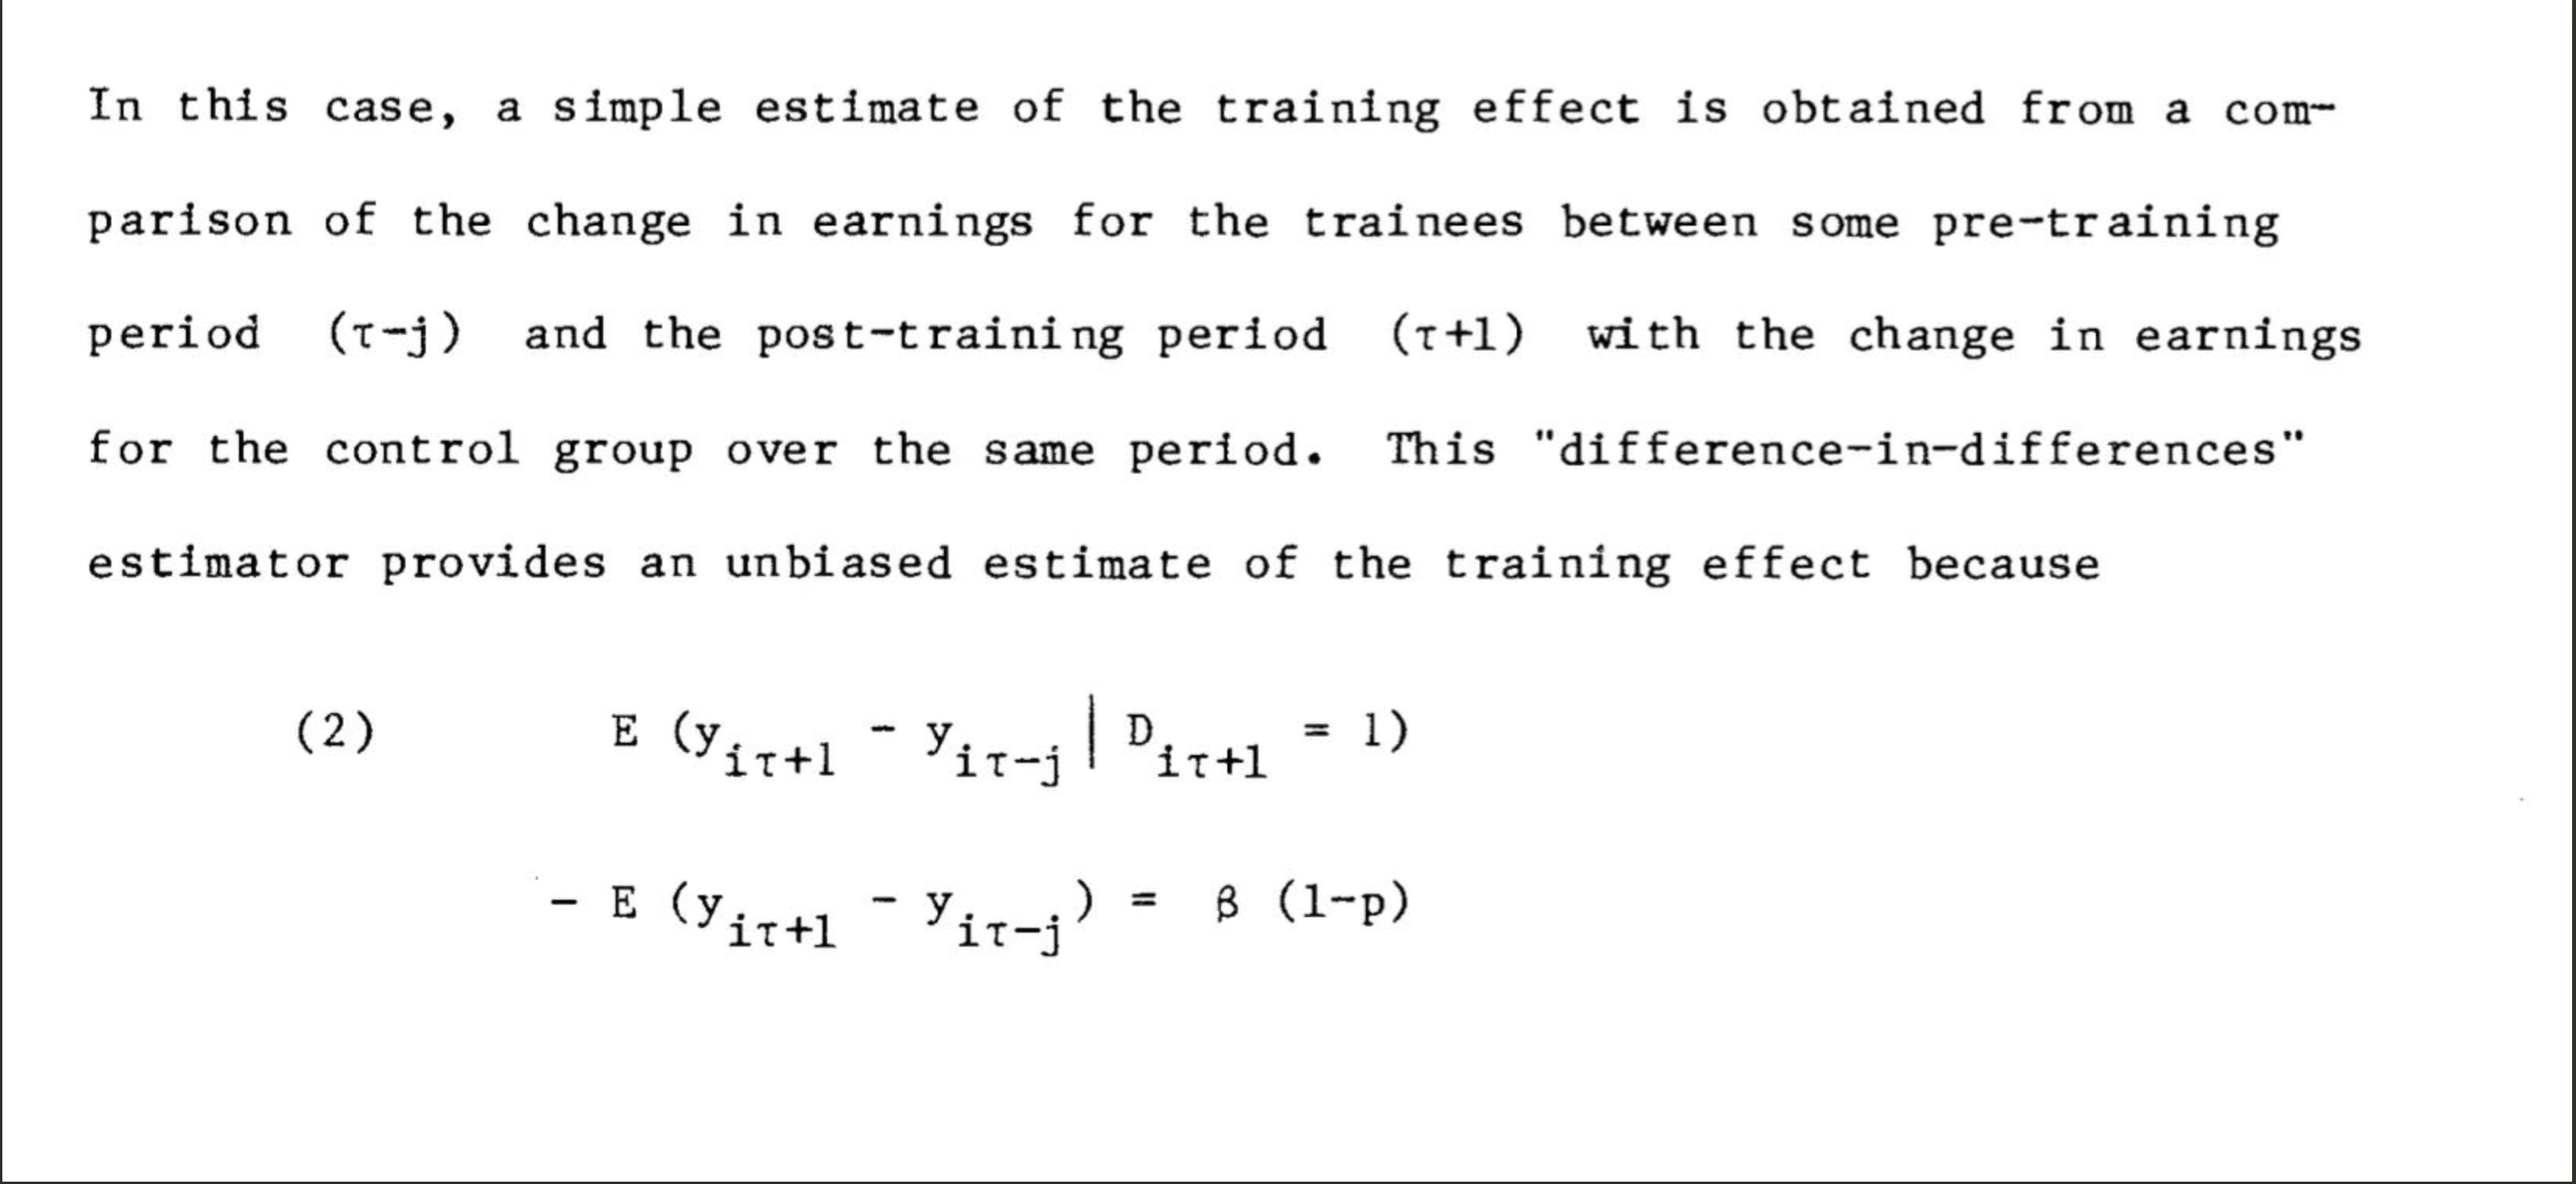
\includegraphics[scale=0.2]{./lecture_includes/orley1983.png}
	\end{figure}


\end{frame}




\begin{frame}{Card on Dips and Parallel Trends}

\begin{itemize}

\item Ashenfelter's Dip is closely linked to difference-in-differences methodology
\item Signs of selection bias visible in time series data between two groups when sudden break from common trend for treatment group just prior to treatment
\item Usually sign of economic distress -- Heckman calls it the Ashenfelter dip
\item Card links it to parallel trends and modern event studies \\ \url{https://youtu.be/1soLdywFb_Q?si=PV16tqFJpKgT_S_W&t=3334}
\end{itemize}

\end{frame}


\begin{frame}{But ``parallel trends'' is nowhere in the paper}

	\begin{figure}
	\caption{No mention of parallel trends in Ashenfelter and Card (1985)}
	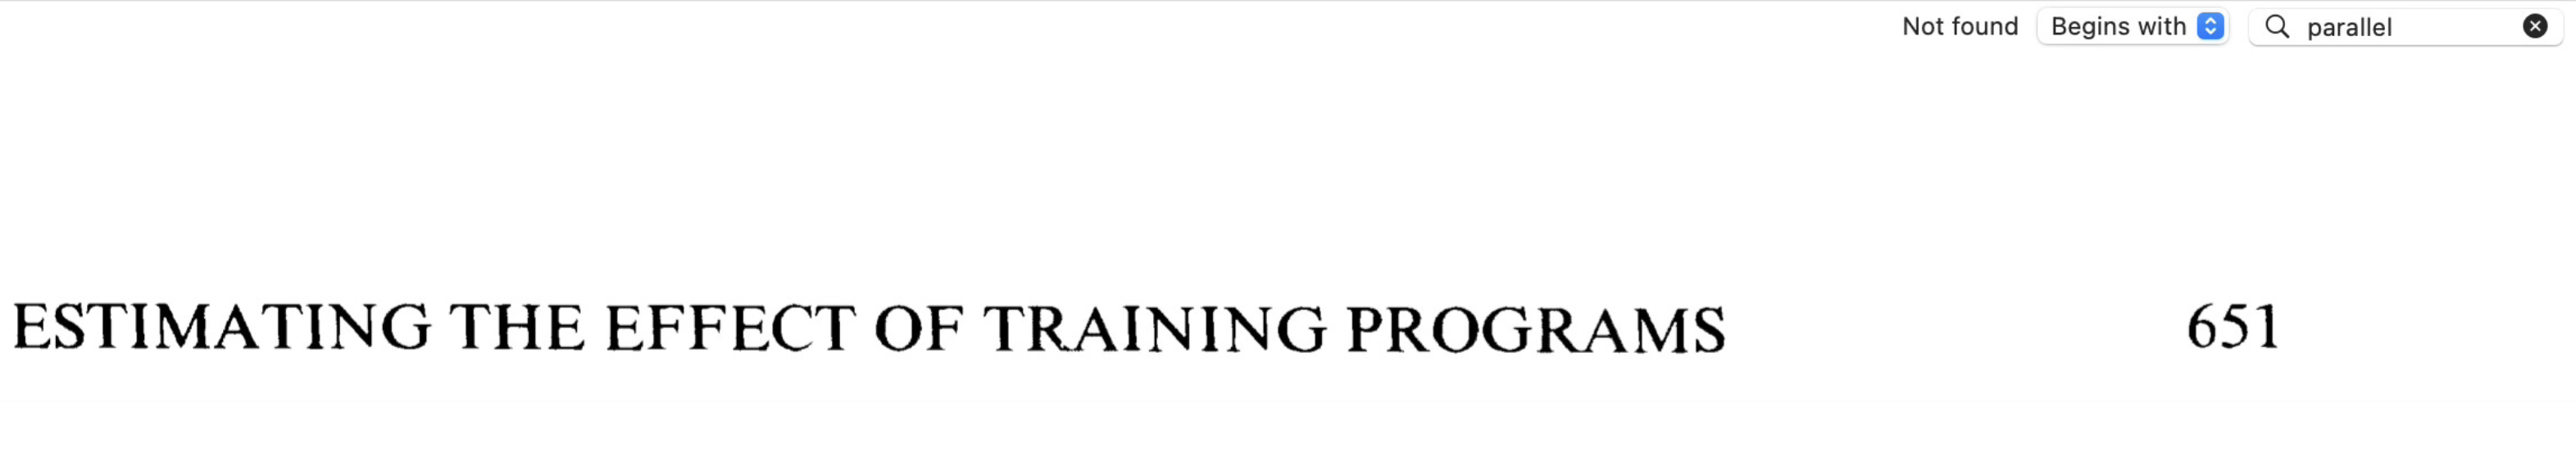
\includegraphics[scale=0.2]{./lecture_includes/nomention.png}
	\end{figure}

\end{frame}




\begin{frame}{Second wave grows faster than first}

\begin{itemize}
\item Share of NBER working papers that used diff-in-diff went from 11-12\% in 2011 to 23\% in 2018, or 11 percentage points
\item It had taken 24 years to reach 11\% the first time, but only 7 years the second time. 
\item 2011 marks the start of the second wave and it has very clear patterns, including the growing speed of adoption
\item Wave 2 links parallel trends and event studies to difference-in-differences for the first time
\end{itemize}

\end{frame}

\begin{frame}{Diff-in-diff versus event study}

	\begin{figure}
	\caption{Currie, et al. (2020)}
	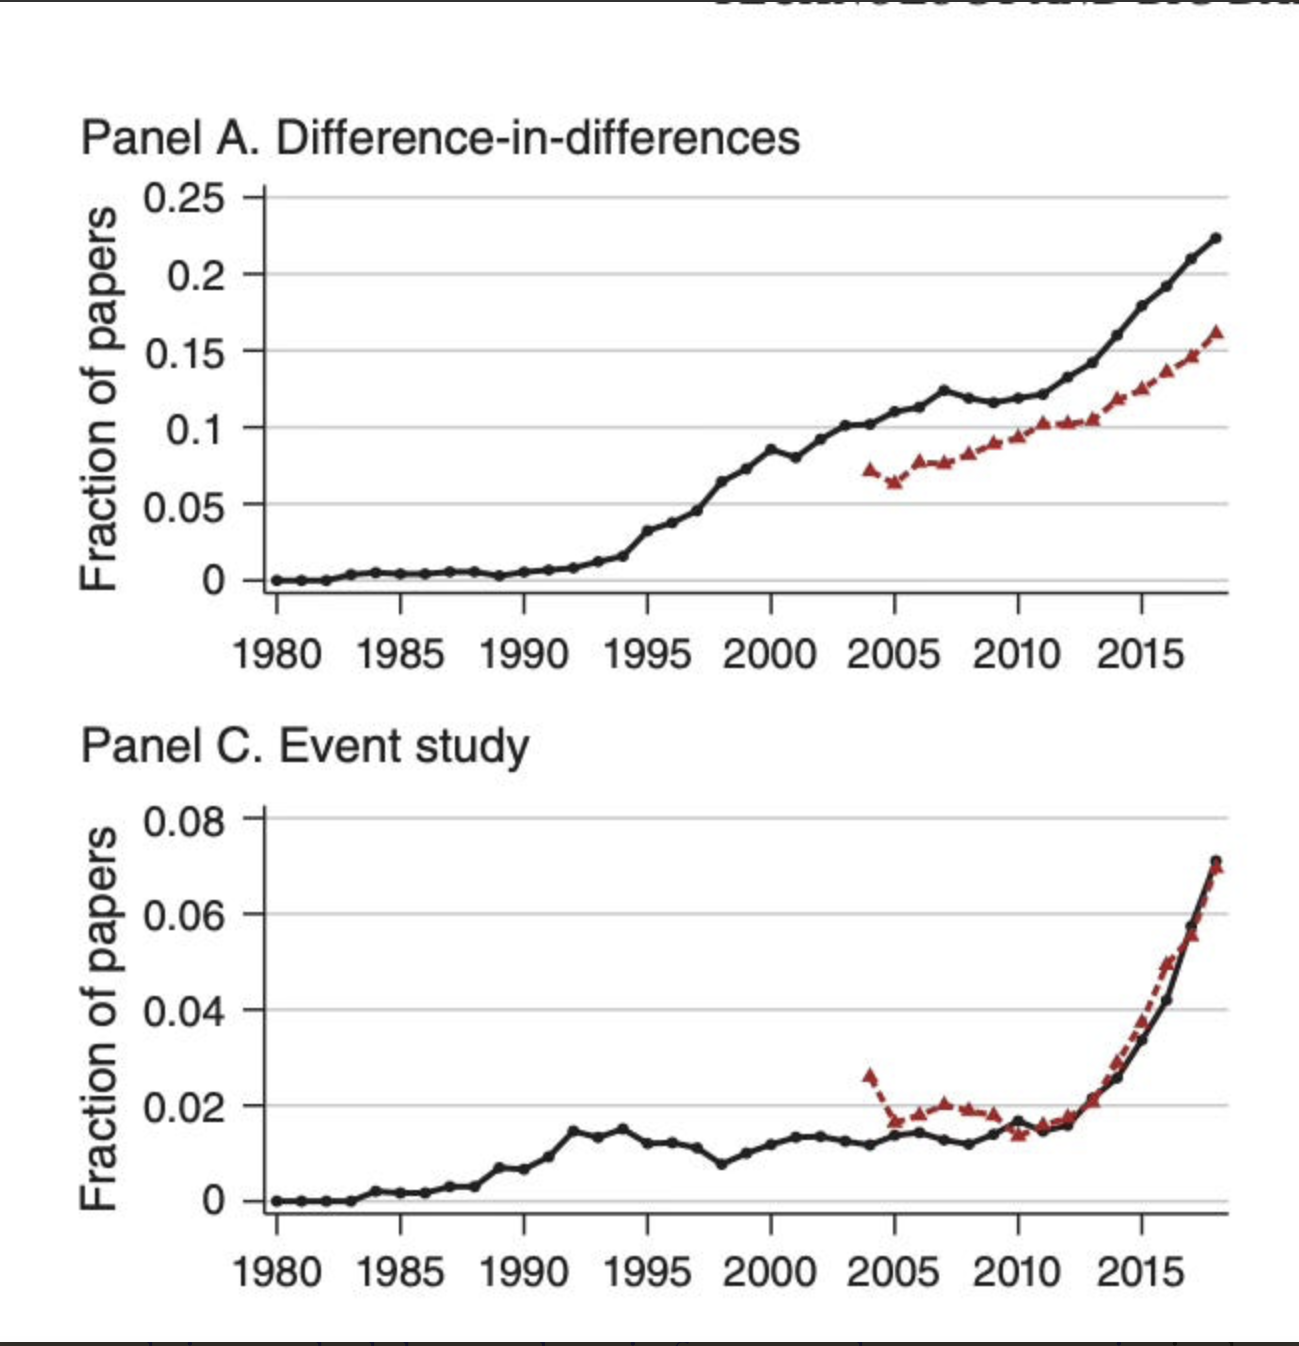
\includegraphics[scale=0.25]{./lecture_includes/secondwave.png}
	\end{figure}


\end{frame}

\begin{frame}{Second wave incorporates parallel trends and event studies}

\begin{itemize}

\item Prior to 2011, authors did not mention "parallel trends" when writing papers using "difference-in-differences"
\item Nor did they use event studies -- those were solely the domain of finance used to study abnormal stock market returns, not in difference-in-differences papers
\item But starting in 2011, diff-in-diff papers appear mentioning the ``event study'' and/or ``parallel trends''
\item Those papers grow exponentially at a rate of 66\% a year
\end{itemize}

\end{frame}

\begin{frame}{Event study and parallel trends}

	\begin{figure}
	\caption{Exponential growth in both event study and parallel trends}
	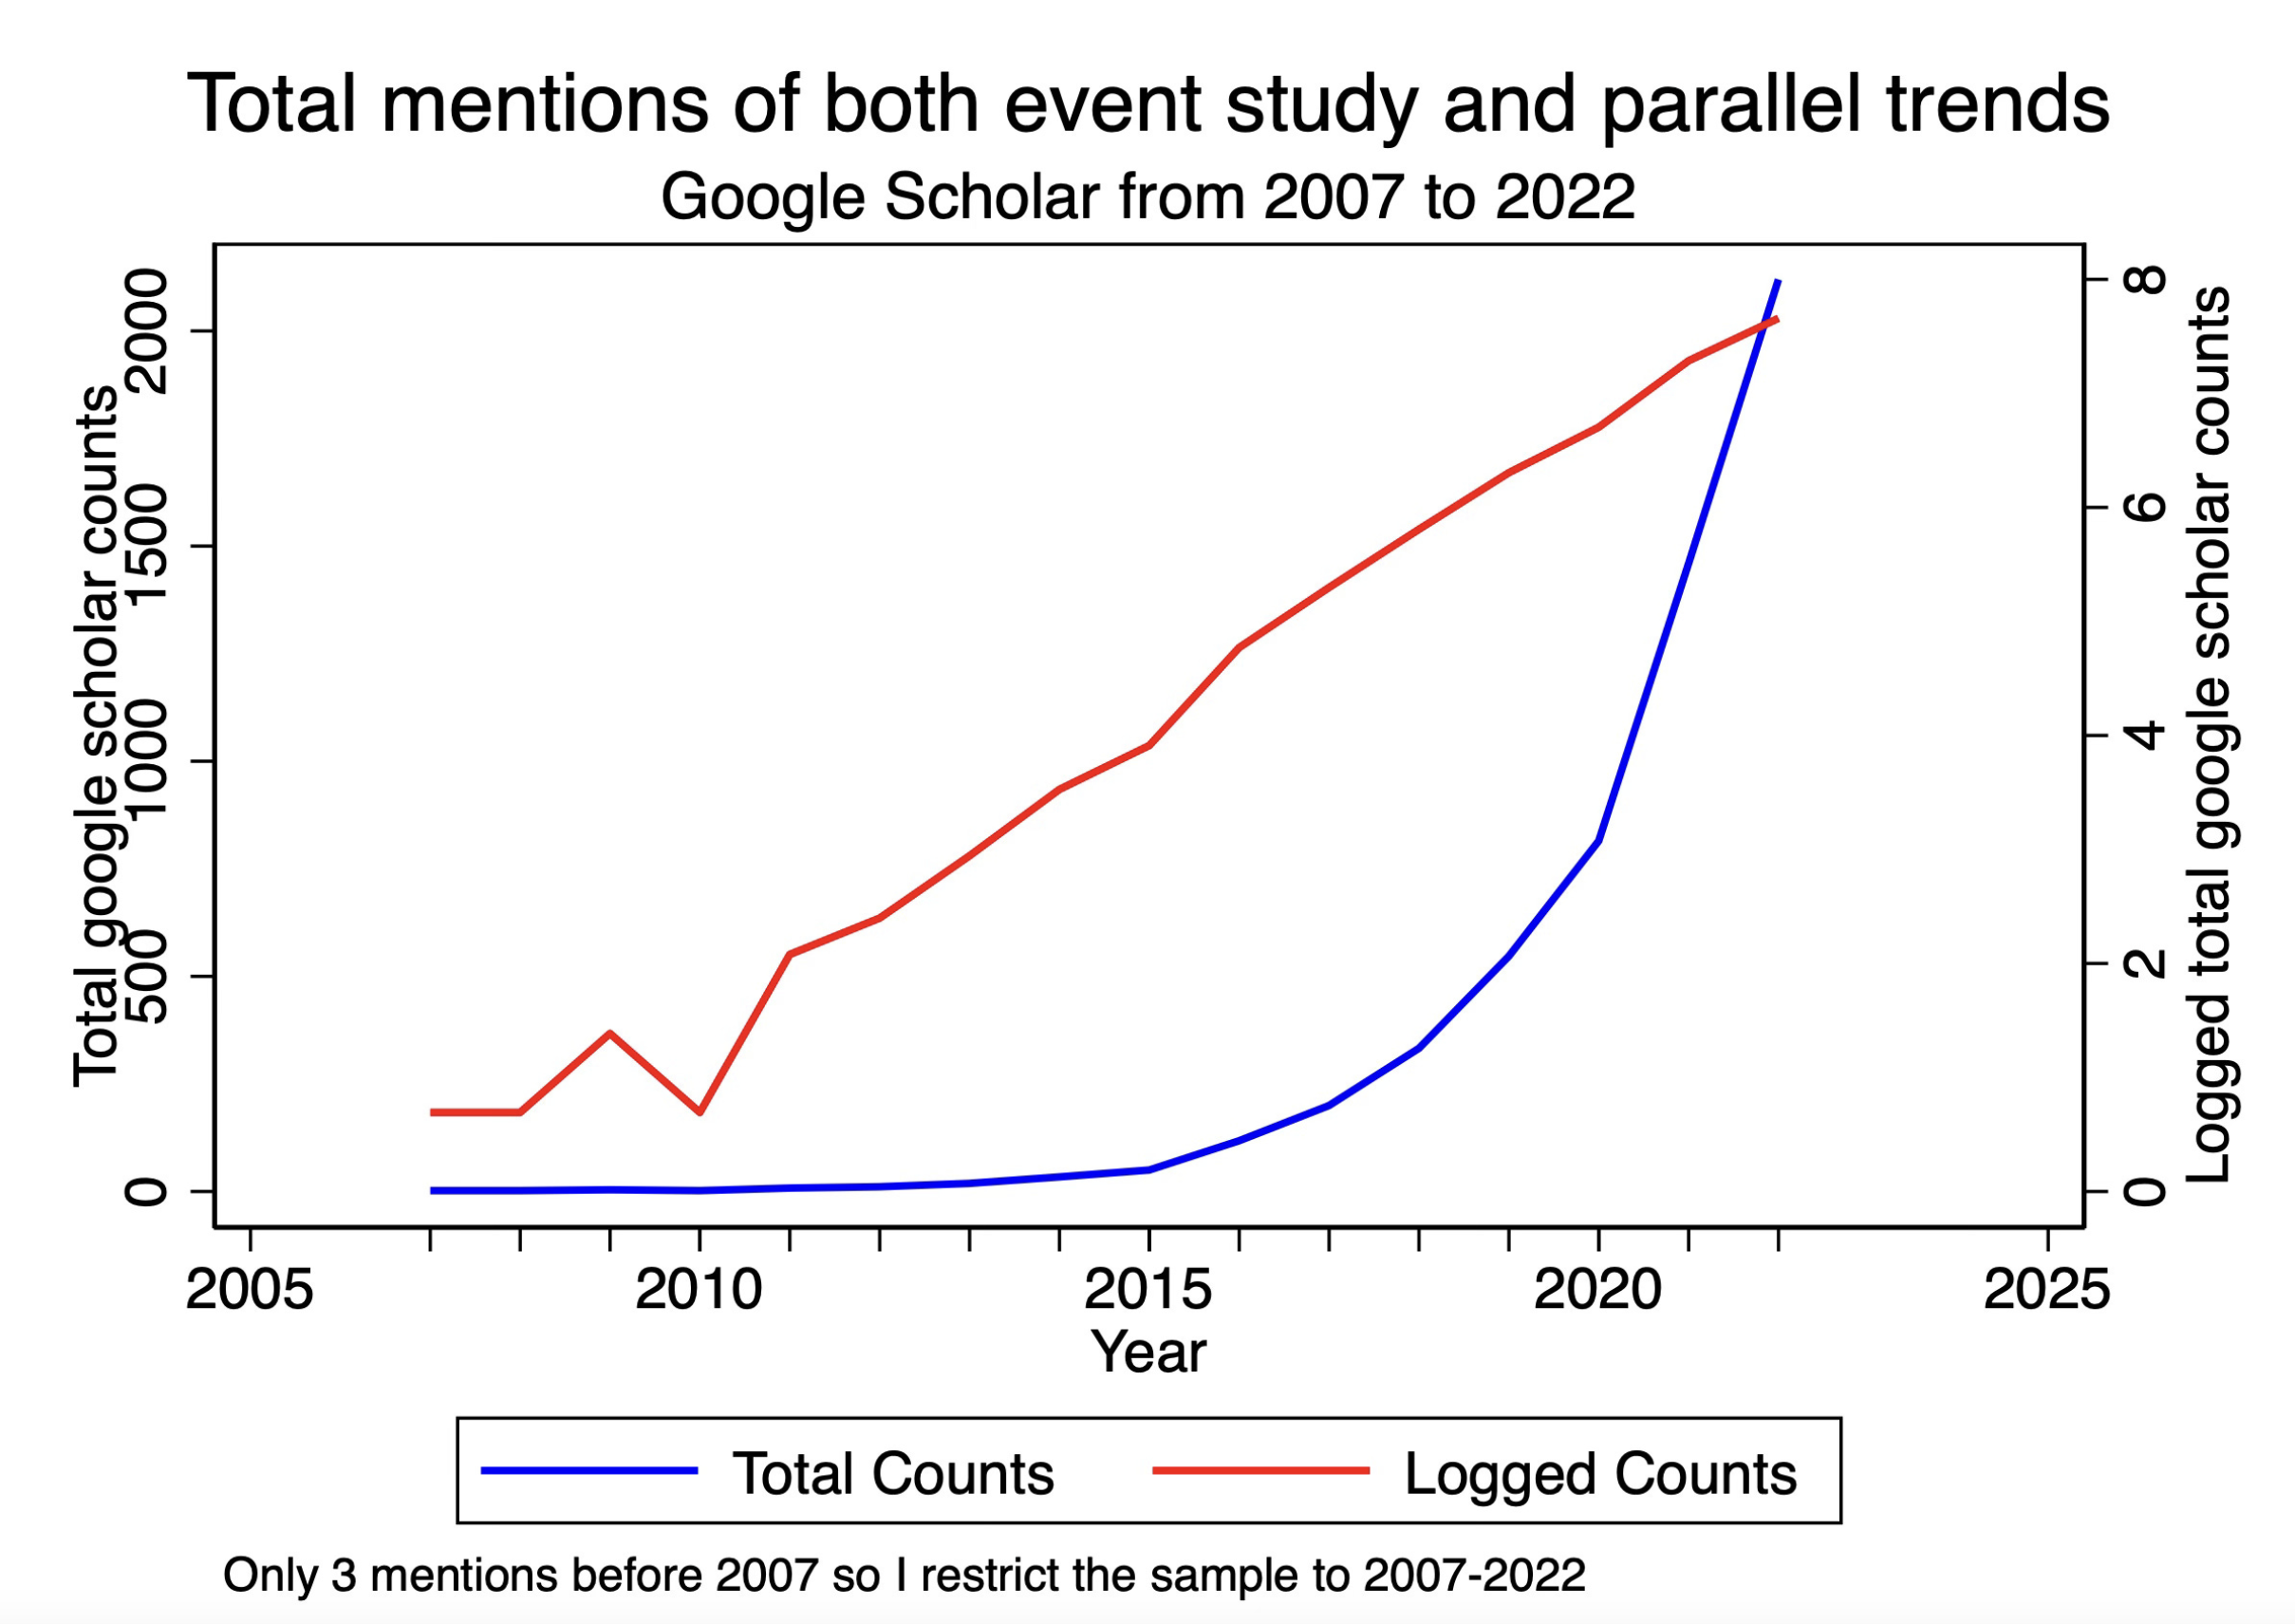
\includegraphics[scale=0.2]{./lecture_includes/event_pt.png}
	\end{figure}

\end{frame}




\begin{frame}{Incorporating PT and event study into diff-in-diff}

	\begin{figure}
	\caption{Growth in both event study and parallel trends}
	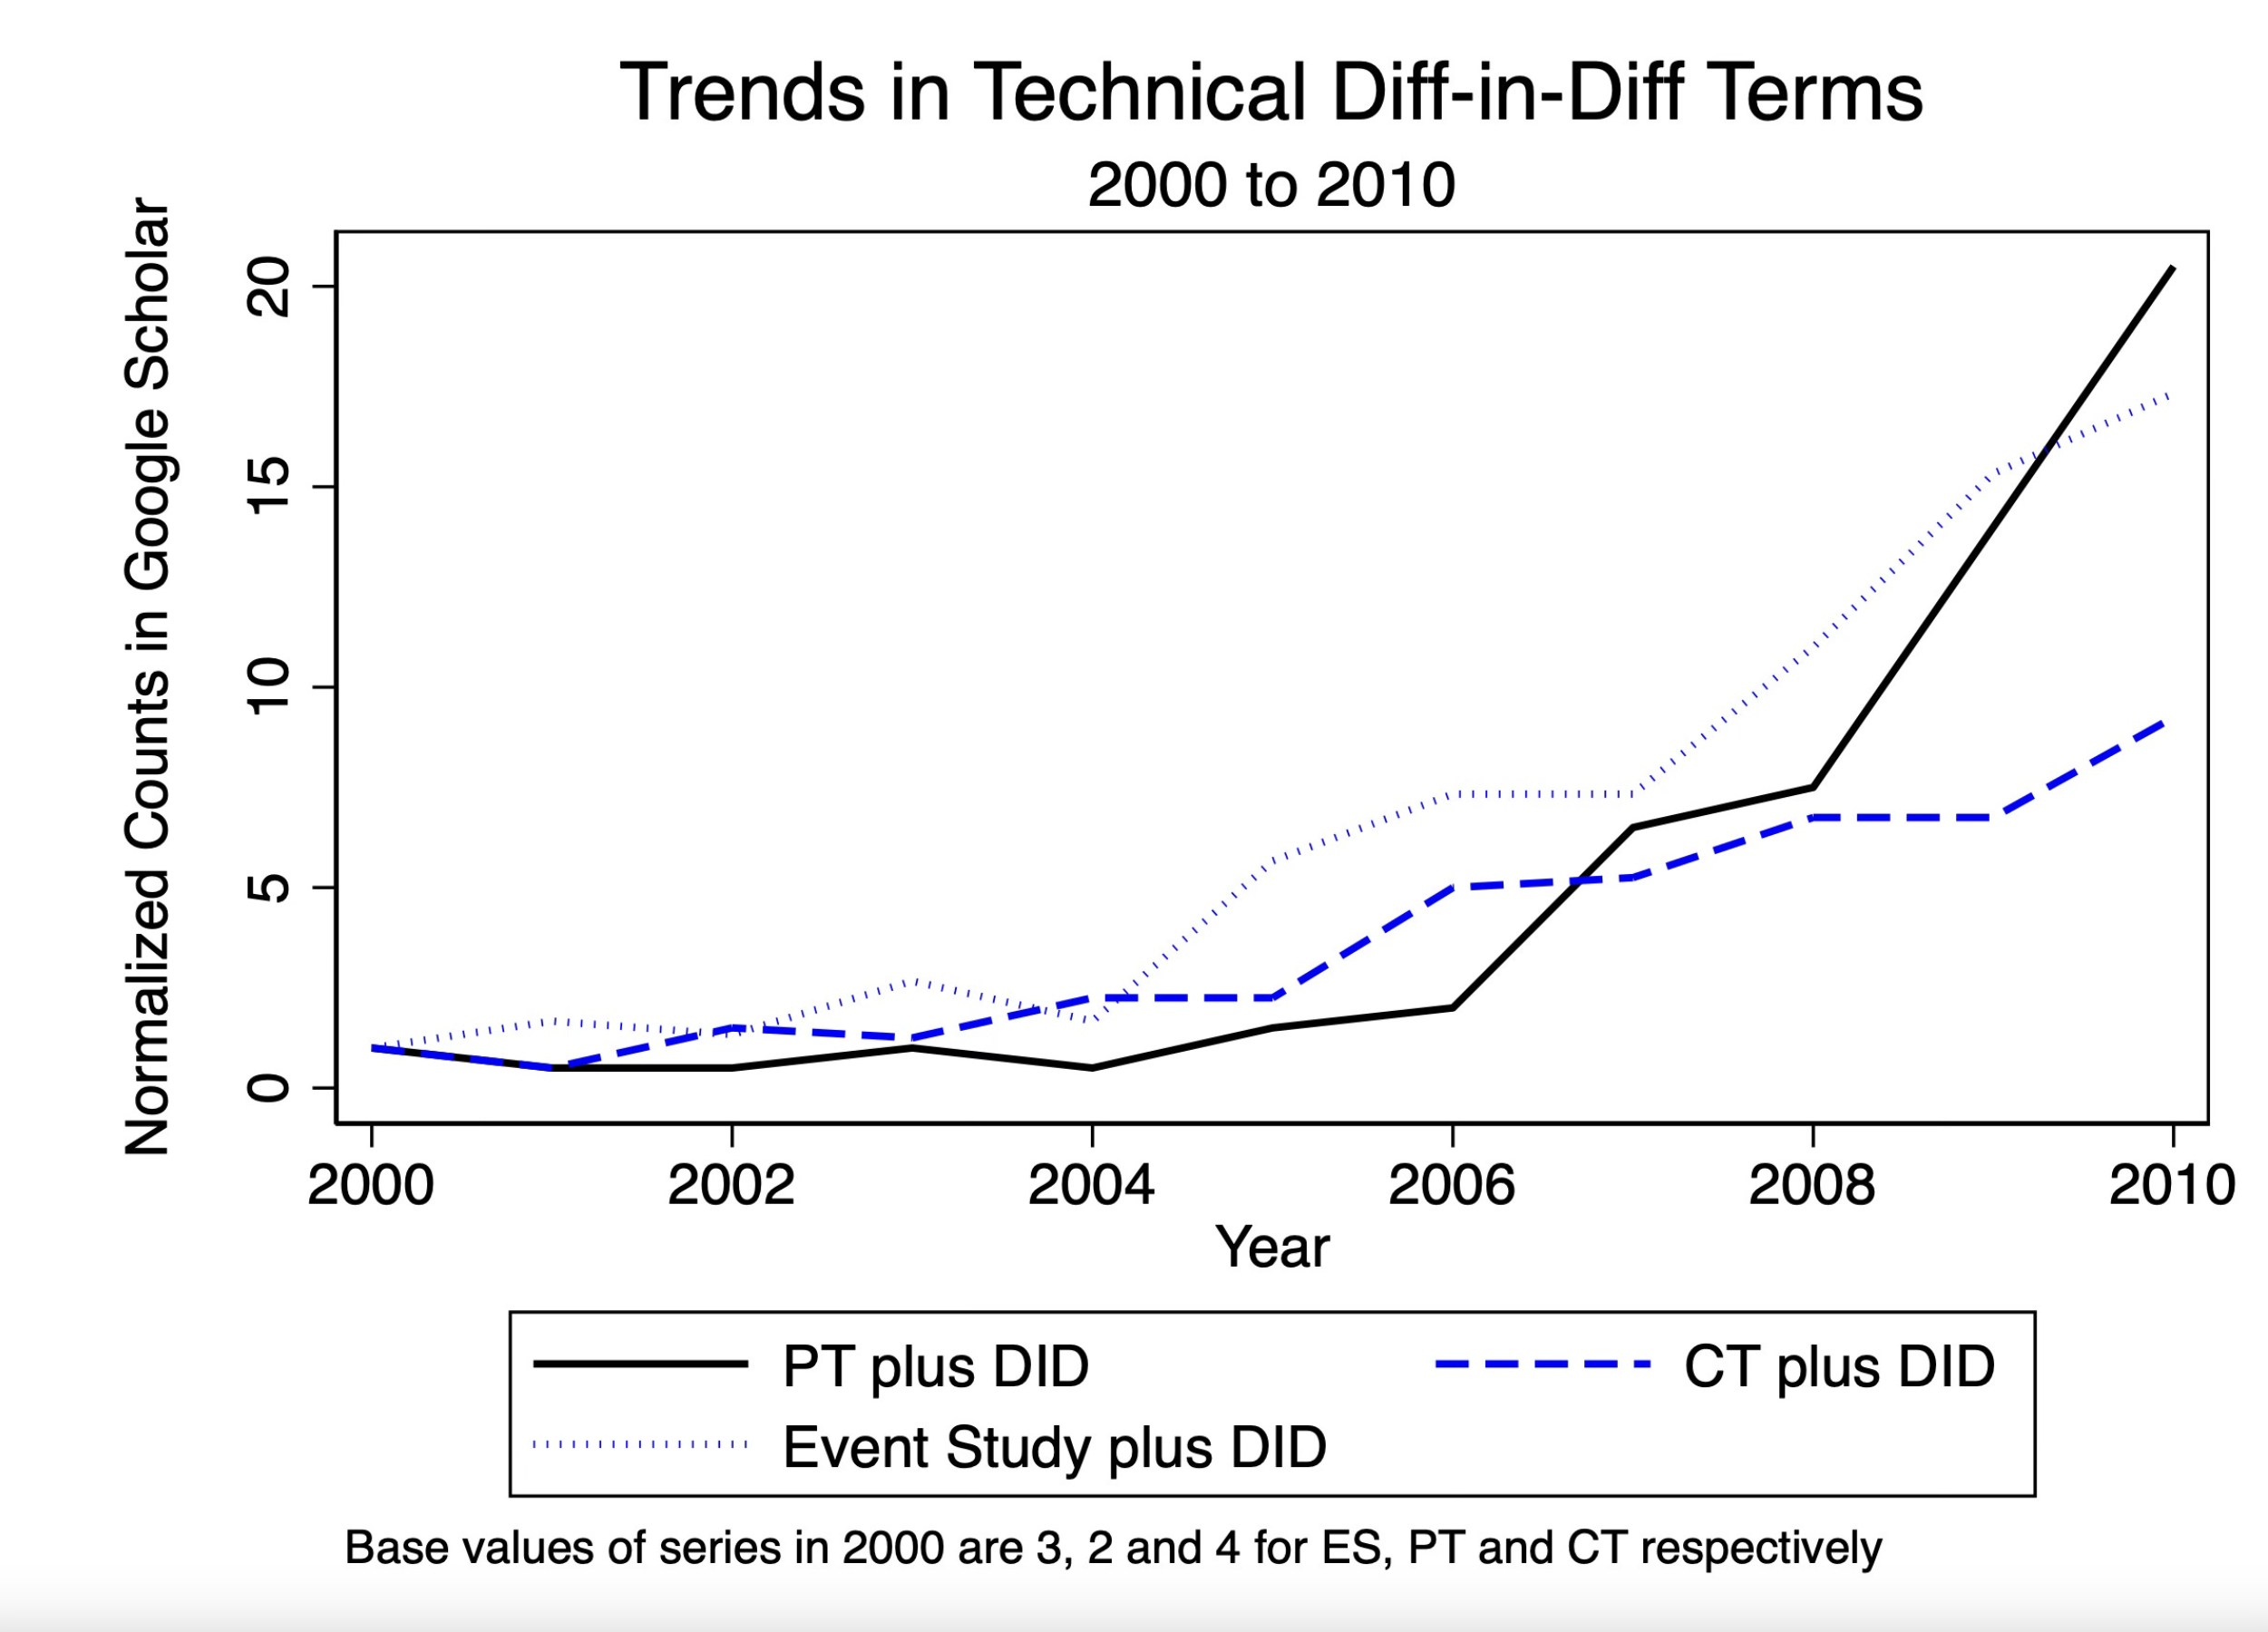
\includegraphics[scale=0.2]{./lecture_includes/espt_2}
	\end{figure}


\end{frame}

\begin{frame}{Incorporating PT and event study into diff-in-diff}

	\begin{figure}
	\caption{Growth in both event study and parallel trends}
	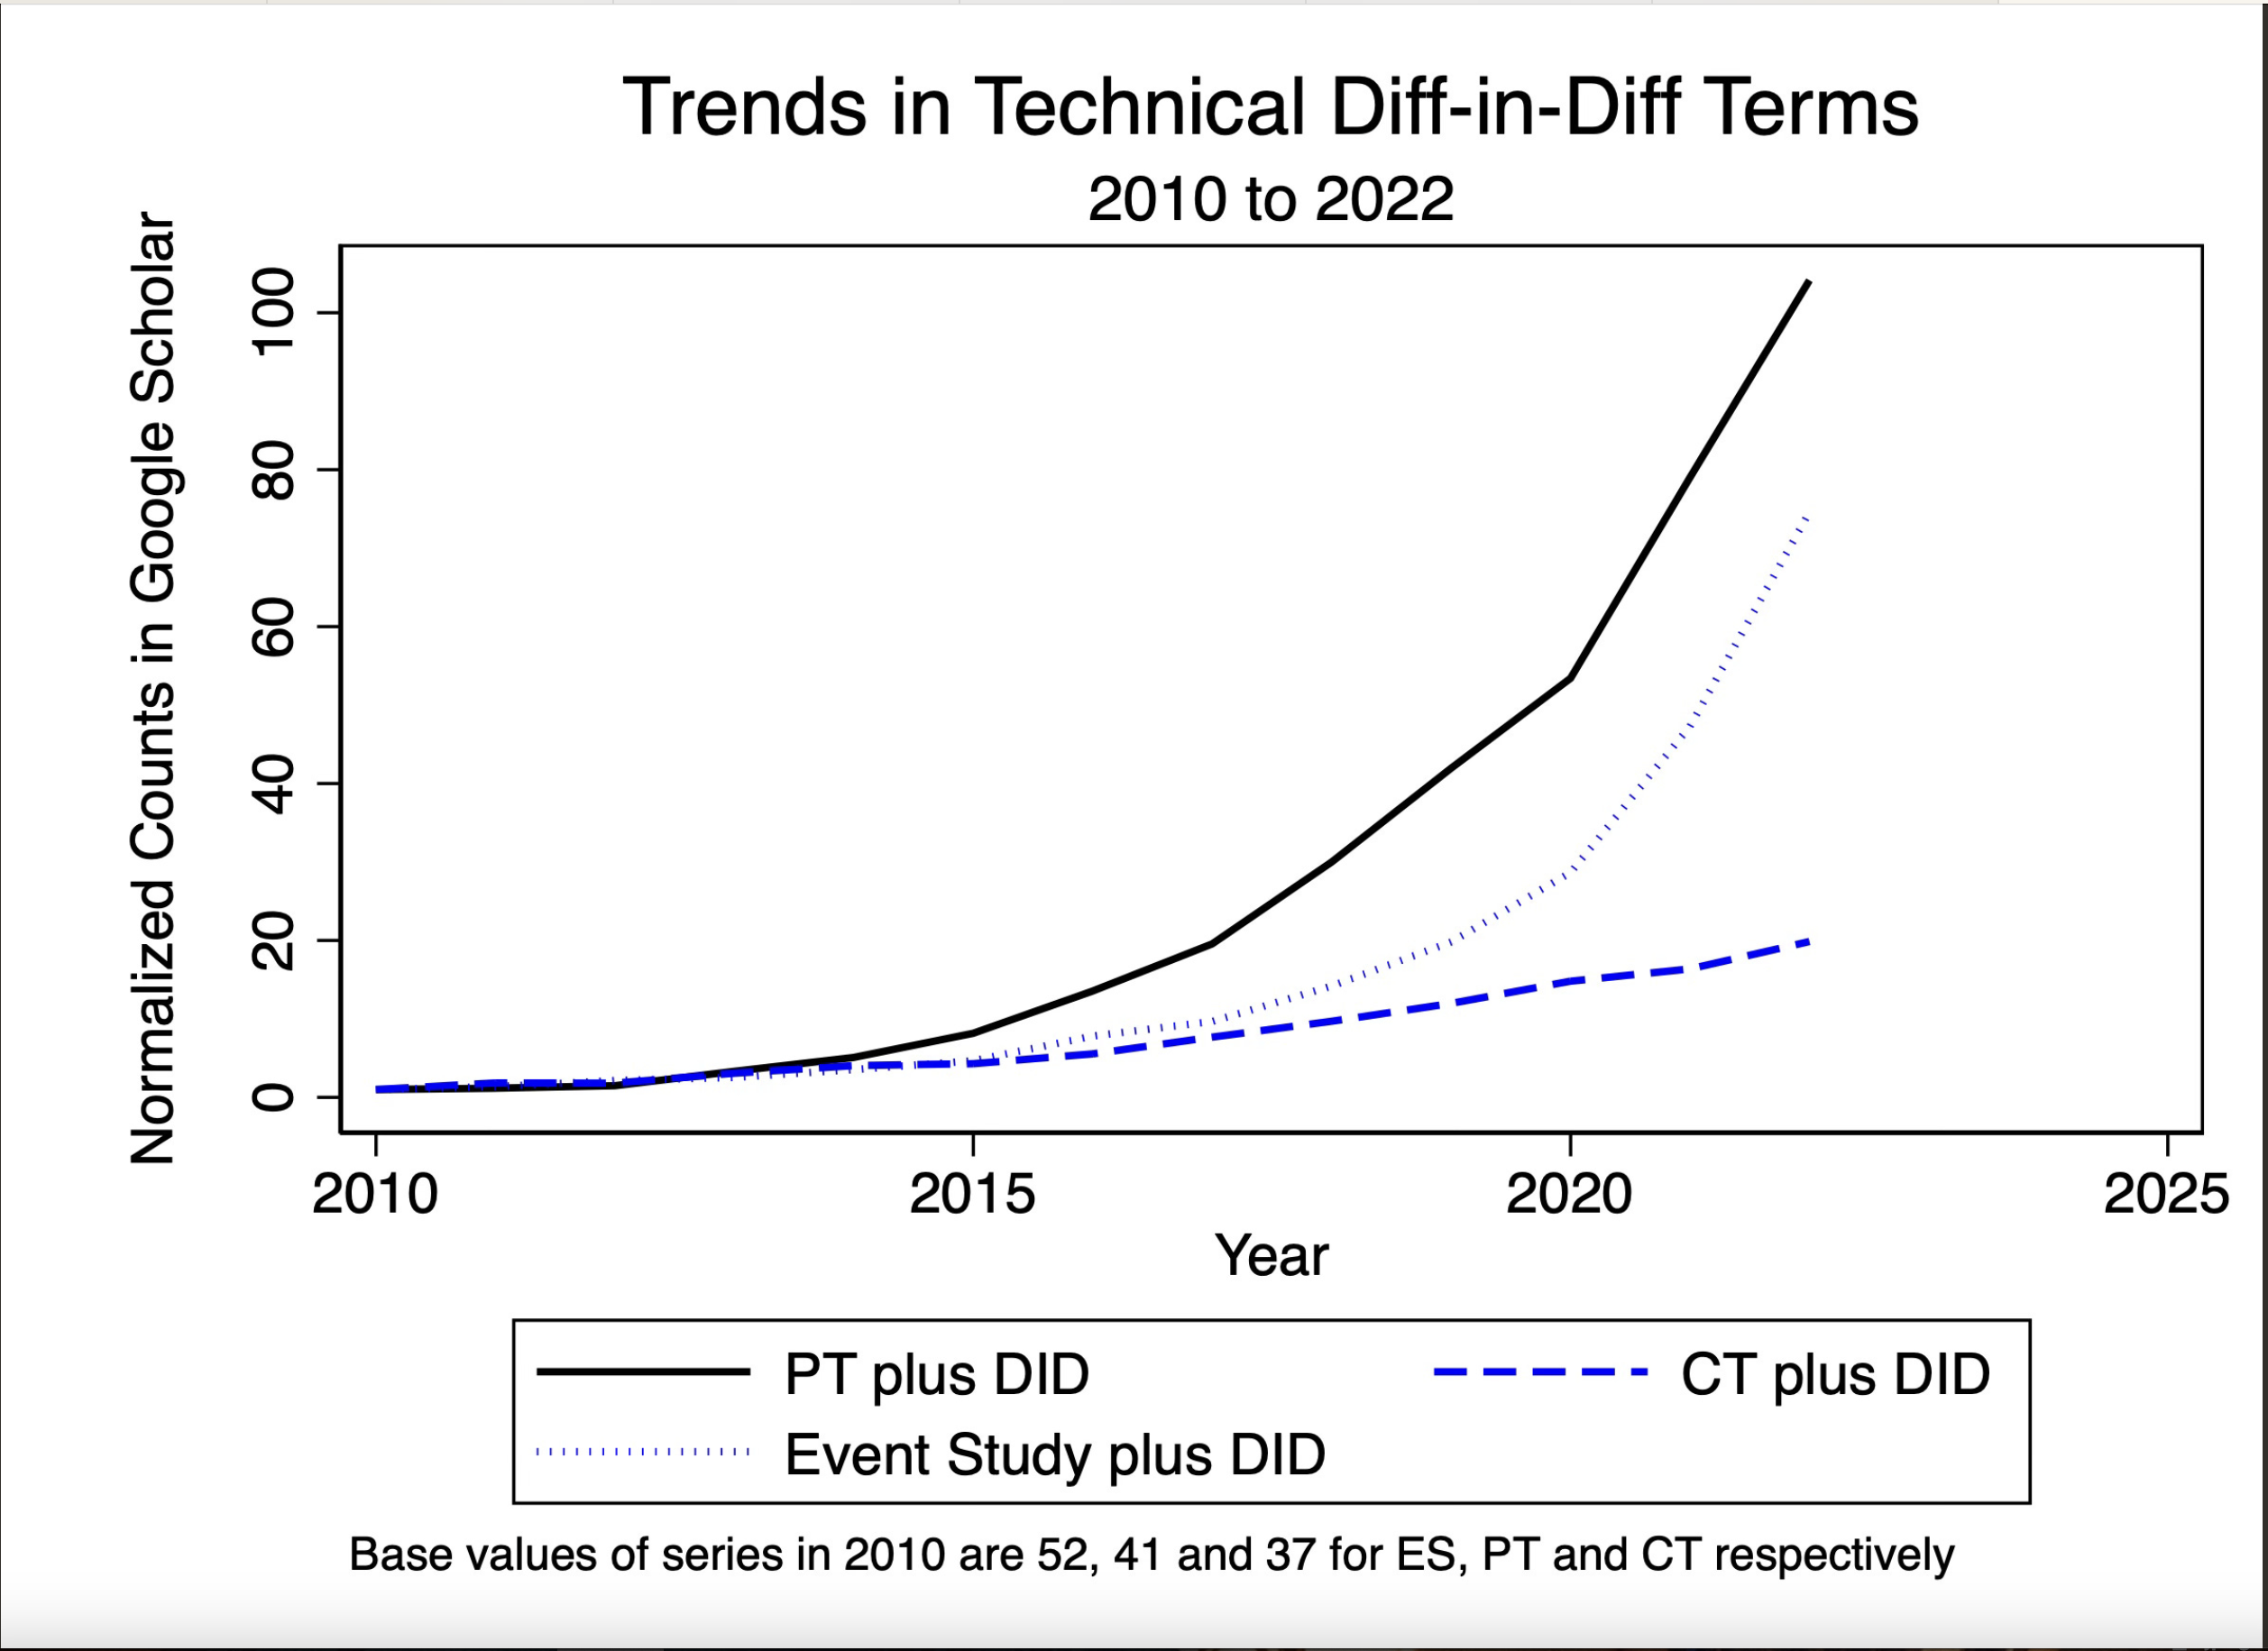
\includegraphics[scale=0.2]{./lecture_includes/espt_3}
	\end{figure}


\end{frame}





\begin{frame}{Parallel trends concept originally meant something else}


 Originally, parallel trends and common trends were synonyms for year fixed effects 
 
 \bigskip
 
	\begin{quote}
	“Moreover, given the increasing dispersion of incomes and wages among all groups during that period, the common time effects (common trends) assumption among the unobservable components across the two groups may not be satisfied.” (Blundell and Dias 1999)
	\end{quote}


\end{frame}

\begin{frame}{Identification shifts away from strict exogeneity}


 Early identification by Blundell was a form of strict exogeneity based panel data (twoway fixed effects), but this was viewed as too strong by Athey and Imbens (2006) 
 
 \bigskip

\begin{quote}
“Note that the full independence assumption $\varepsilon_i \independent(G_i,T_i)$ (e.g., Blundell and MaCurdy (2000)) is stronger than necessary for [DiD] to give the average treatment effect.”
\end{quote}


\end{frame}



\begin{frame}{Heckman, et al. (1997) introduce potenial outcomes}


\begin{itemize}
\item Heckman, Ichimura and Todd (1997) introduce both \emph{conditional} parallel trends and potential outcomes for identification in difference-in-differences (but not the phrase)

\bigskip

	\begin{figure}
	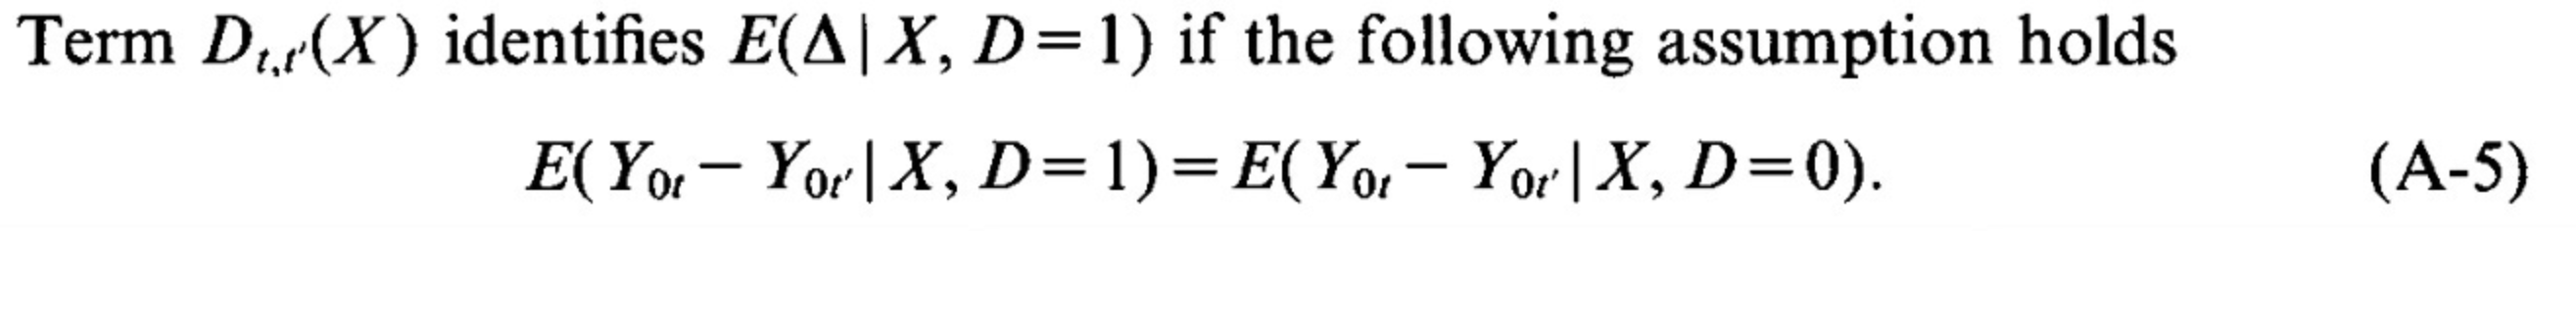
\includegraphics[scale=0.2]{./lecture_includes/heckman_cpt}
	\end{figure}


\item Angrist and Pischke (2009) chapter 5 is entitled "Parallel Worlds: Fixed Effects, Difference-in-Differences and Panel Data''
\item Though the phrase ``parallel trends'' does not appear in the book, our earlier time series showed PT and DID trends begin rising along with event study and DID by the mid to late 00s
\end{itemize}


\end{frame}




\begin{frame}{Mostly Harmless and Parallel Trends}


	\begin{figure}
	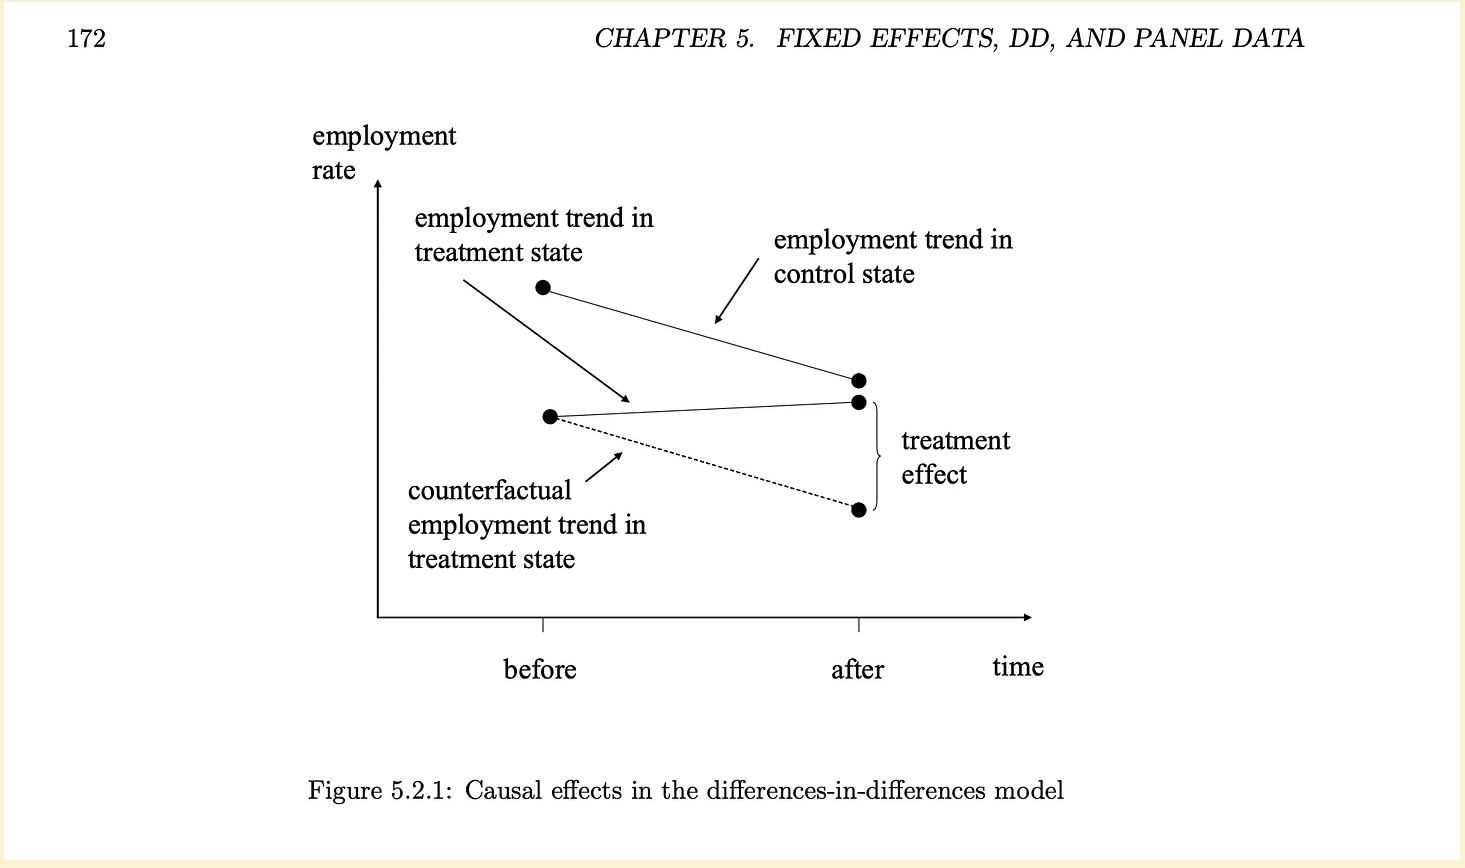
\includegraphics[scale=0.45]{./lecture_includes/mhe_pt}
	\end{figure}



\end{frame}




\begin{frame}{Third wave: heterogeneity and TWFE}

\begin{itemize}

\item Third (and current) wave has been characterized by scrutiny of the twoway fixed effects (TWFE) model starting around 2018
\item Economists were using TWFE because it's a panel estimator and diff-in-diff could be used with panel data (or repeated cross-sections)
\item But subtle assumptions are buried in the details, or not made explicit at all, related to heterogeneous vs constant treatment effects


\end{itemize}

\end{frame}



\begin{frame}{Event Studies and Differential Timing}

	\begin{figure}
	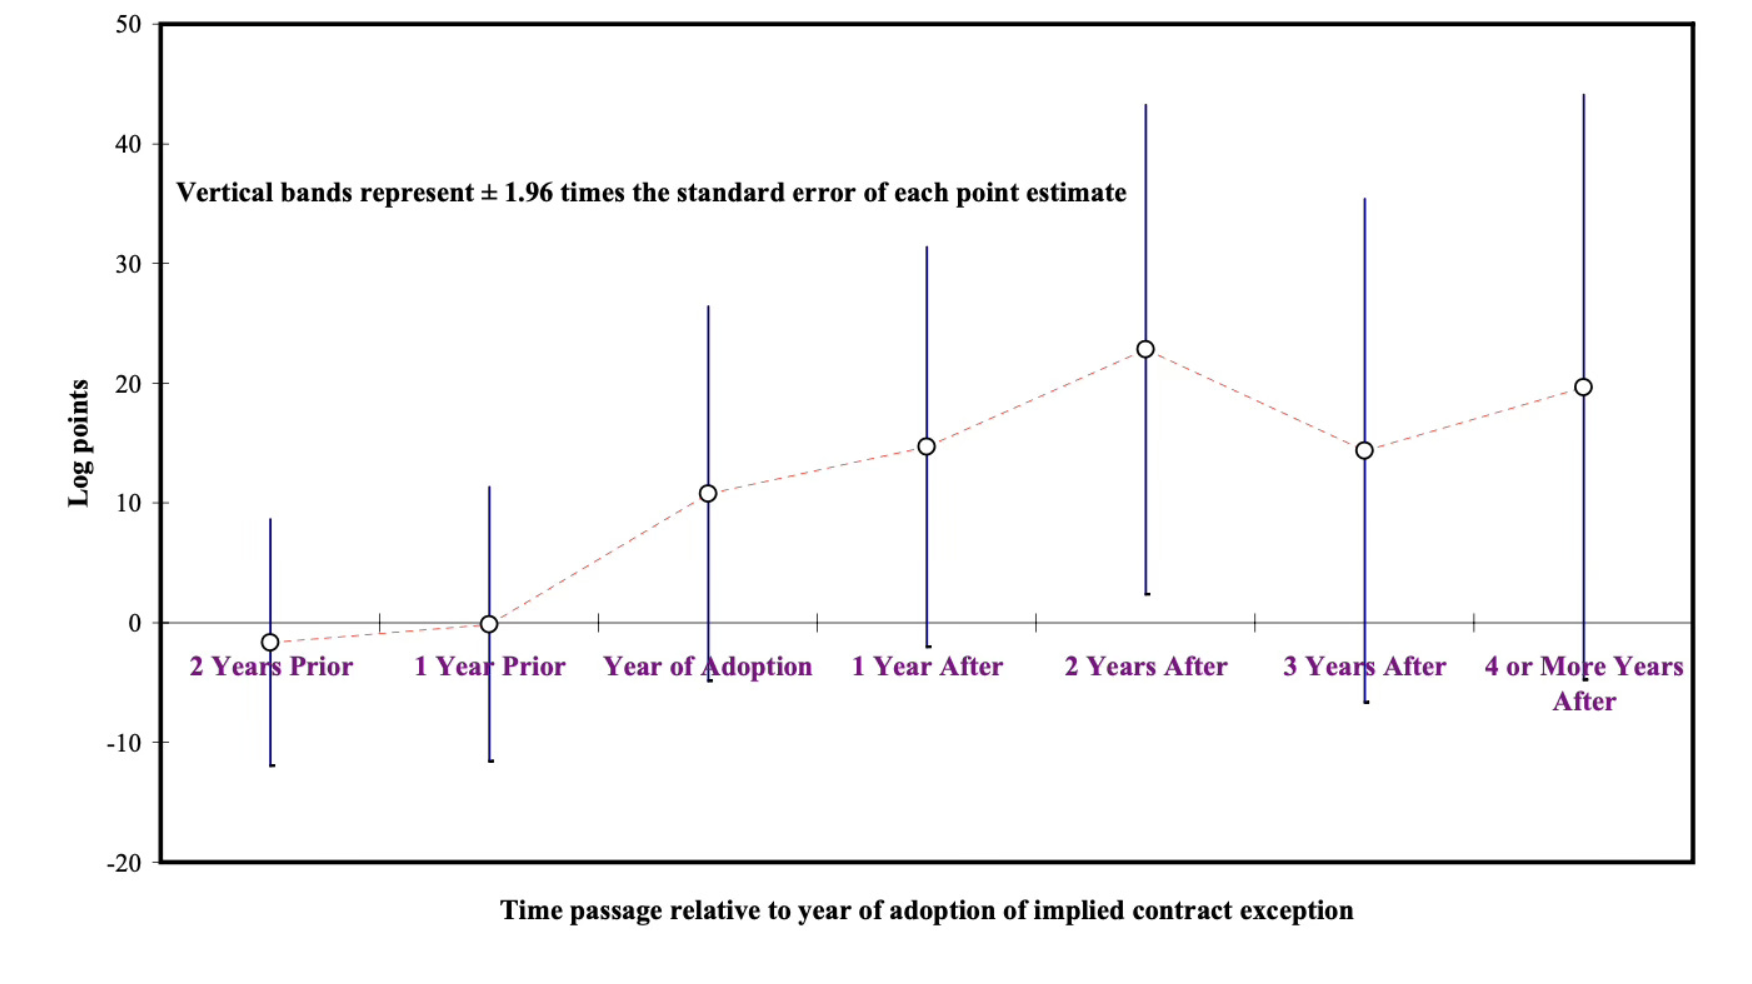
\includegraphics[scale=0.35]{./lecture_includes/autor2003}
	\caption{David Autor (2003) ``unjust dismissals'' paper}
	\end{figure}

\end{frame}

\begin{frame}{Constant effects model}

	\begin{figure}
	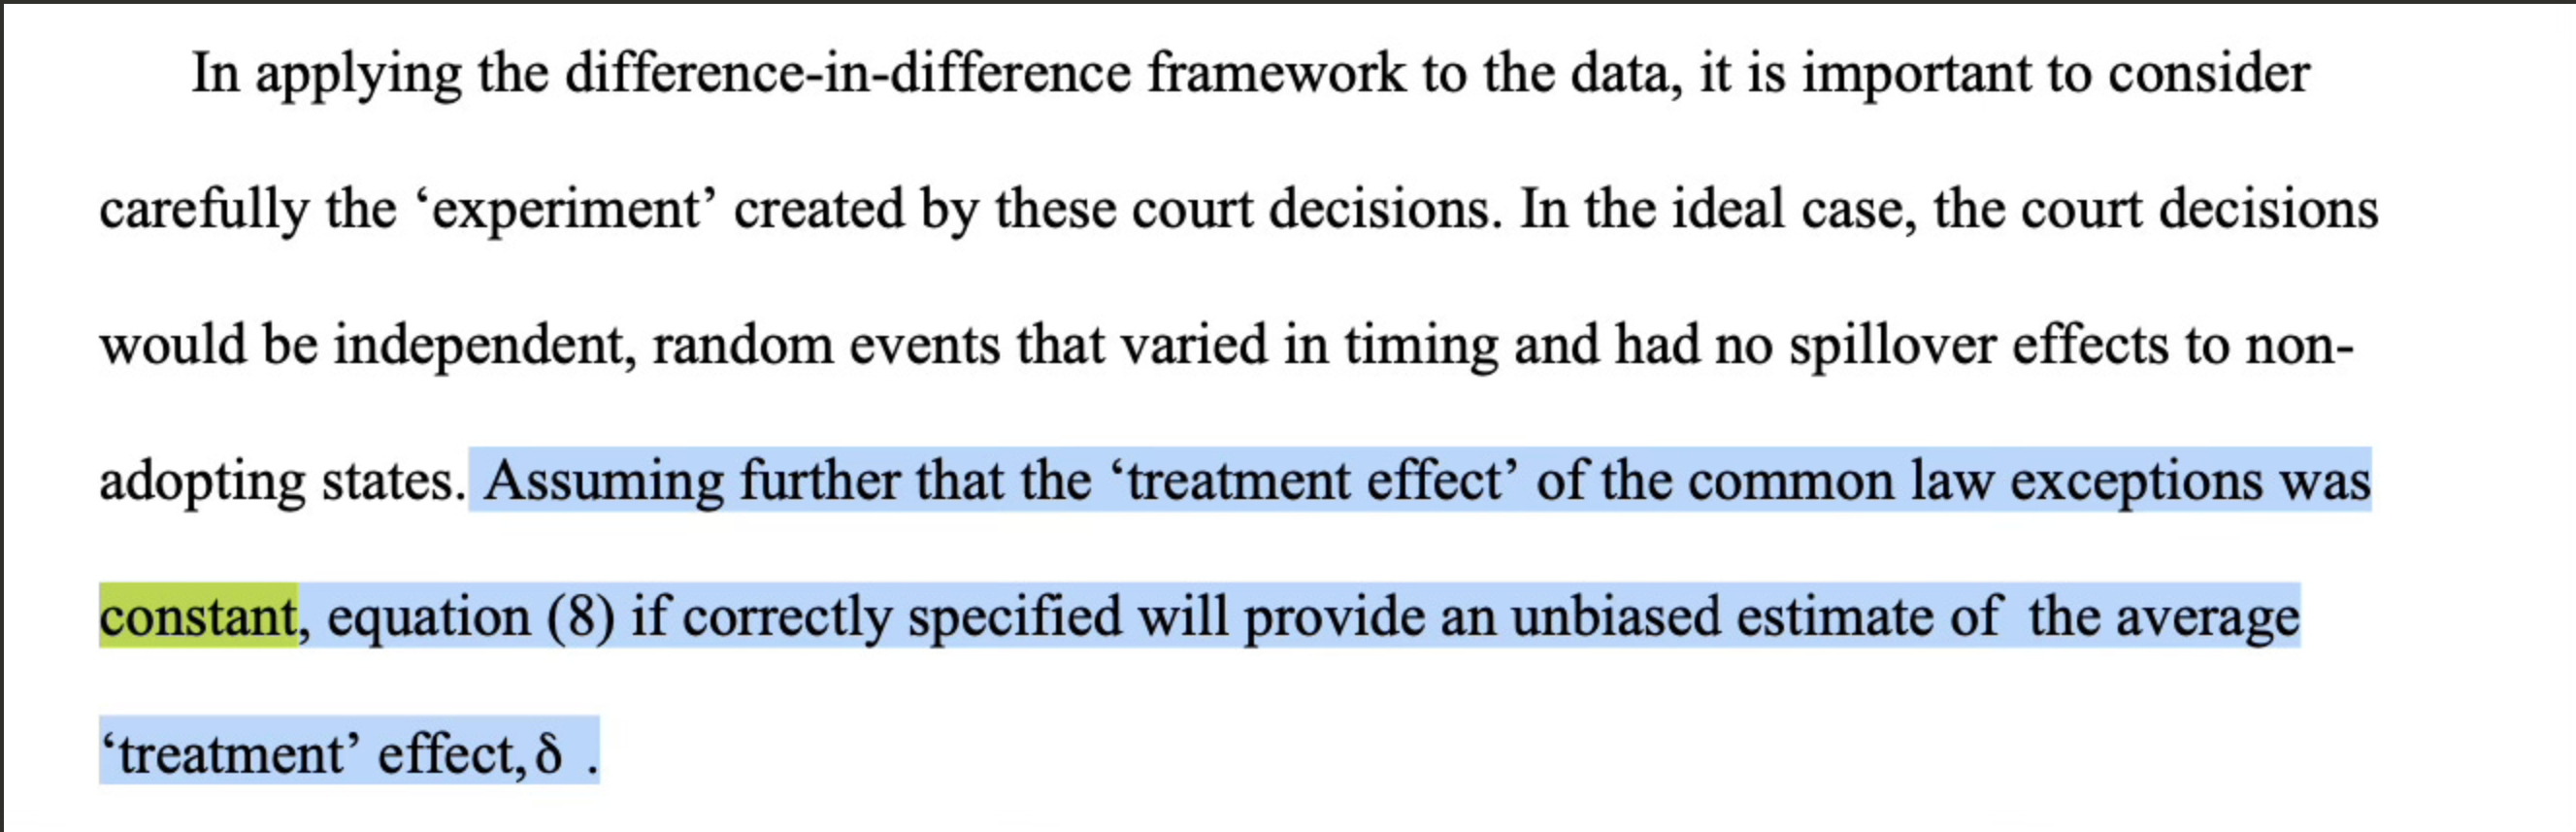
\includegraphics[scale=0.25]{./lecture_includes/autor_quote}
	\caption{David Autor clues us into the problems of TWFE}
	\end{figure}

\end{frame}









\begin{frame}{Third wave of diff-in-diff}

\begin{itemize}

\item Autor (2003) quote echoes down the years as researchers begin to investigate what happens when constant treatment effects is relaxed
\item Starts with Kirill Borusyak and Xavier Jaravel (2016) working paper posted to SSRN (later published with Jan Speiss 2023)
\item Wave 3 links difference-in-differences with heterogenous treatment effects, the pathologies of twoway fixed effects (TWFE) and begins to shift away from TWFE
\end{itemize}

\end{frame}


\begin{frame}{First Wave}

	\begin{figure}
	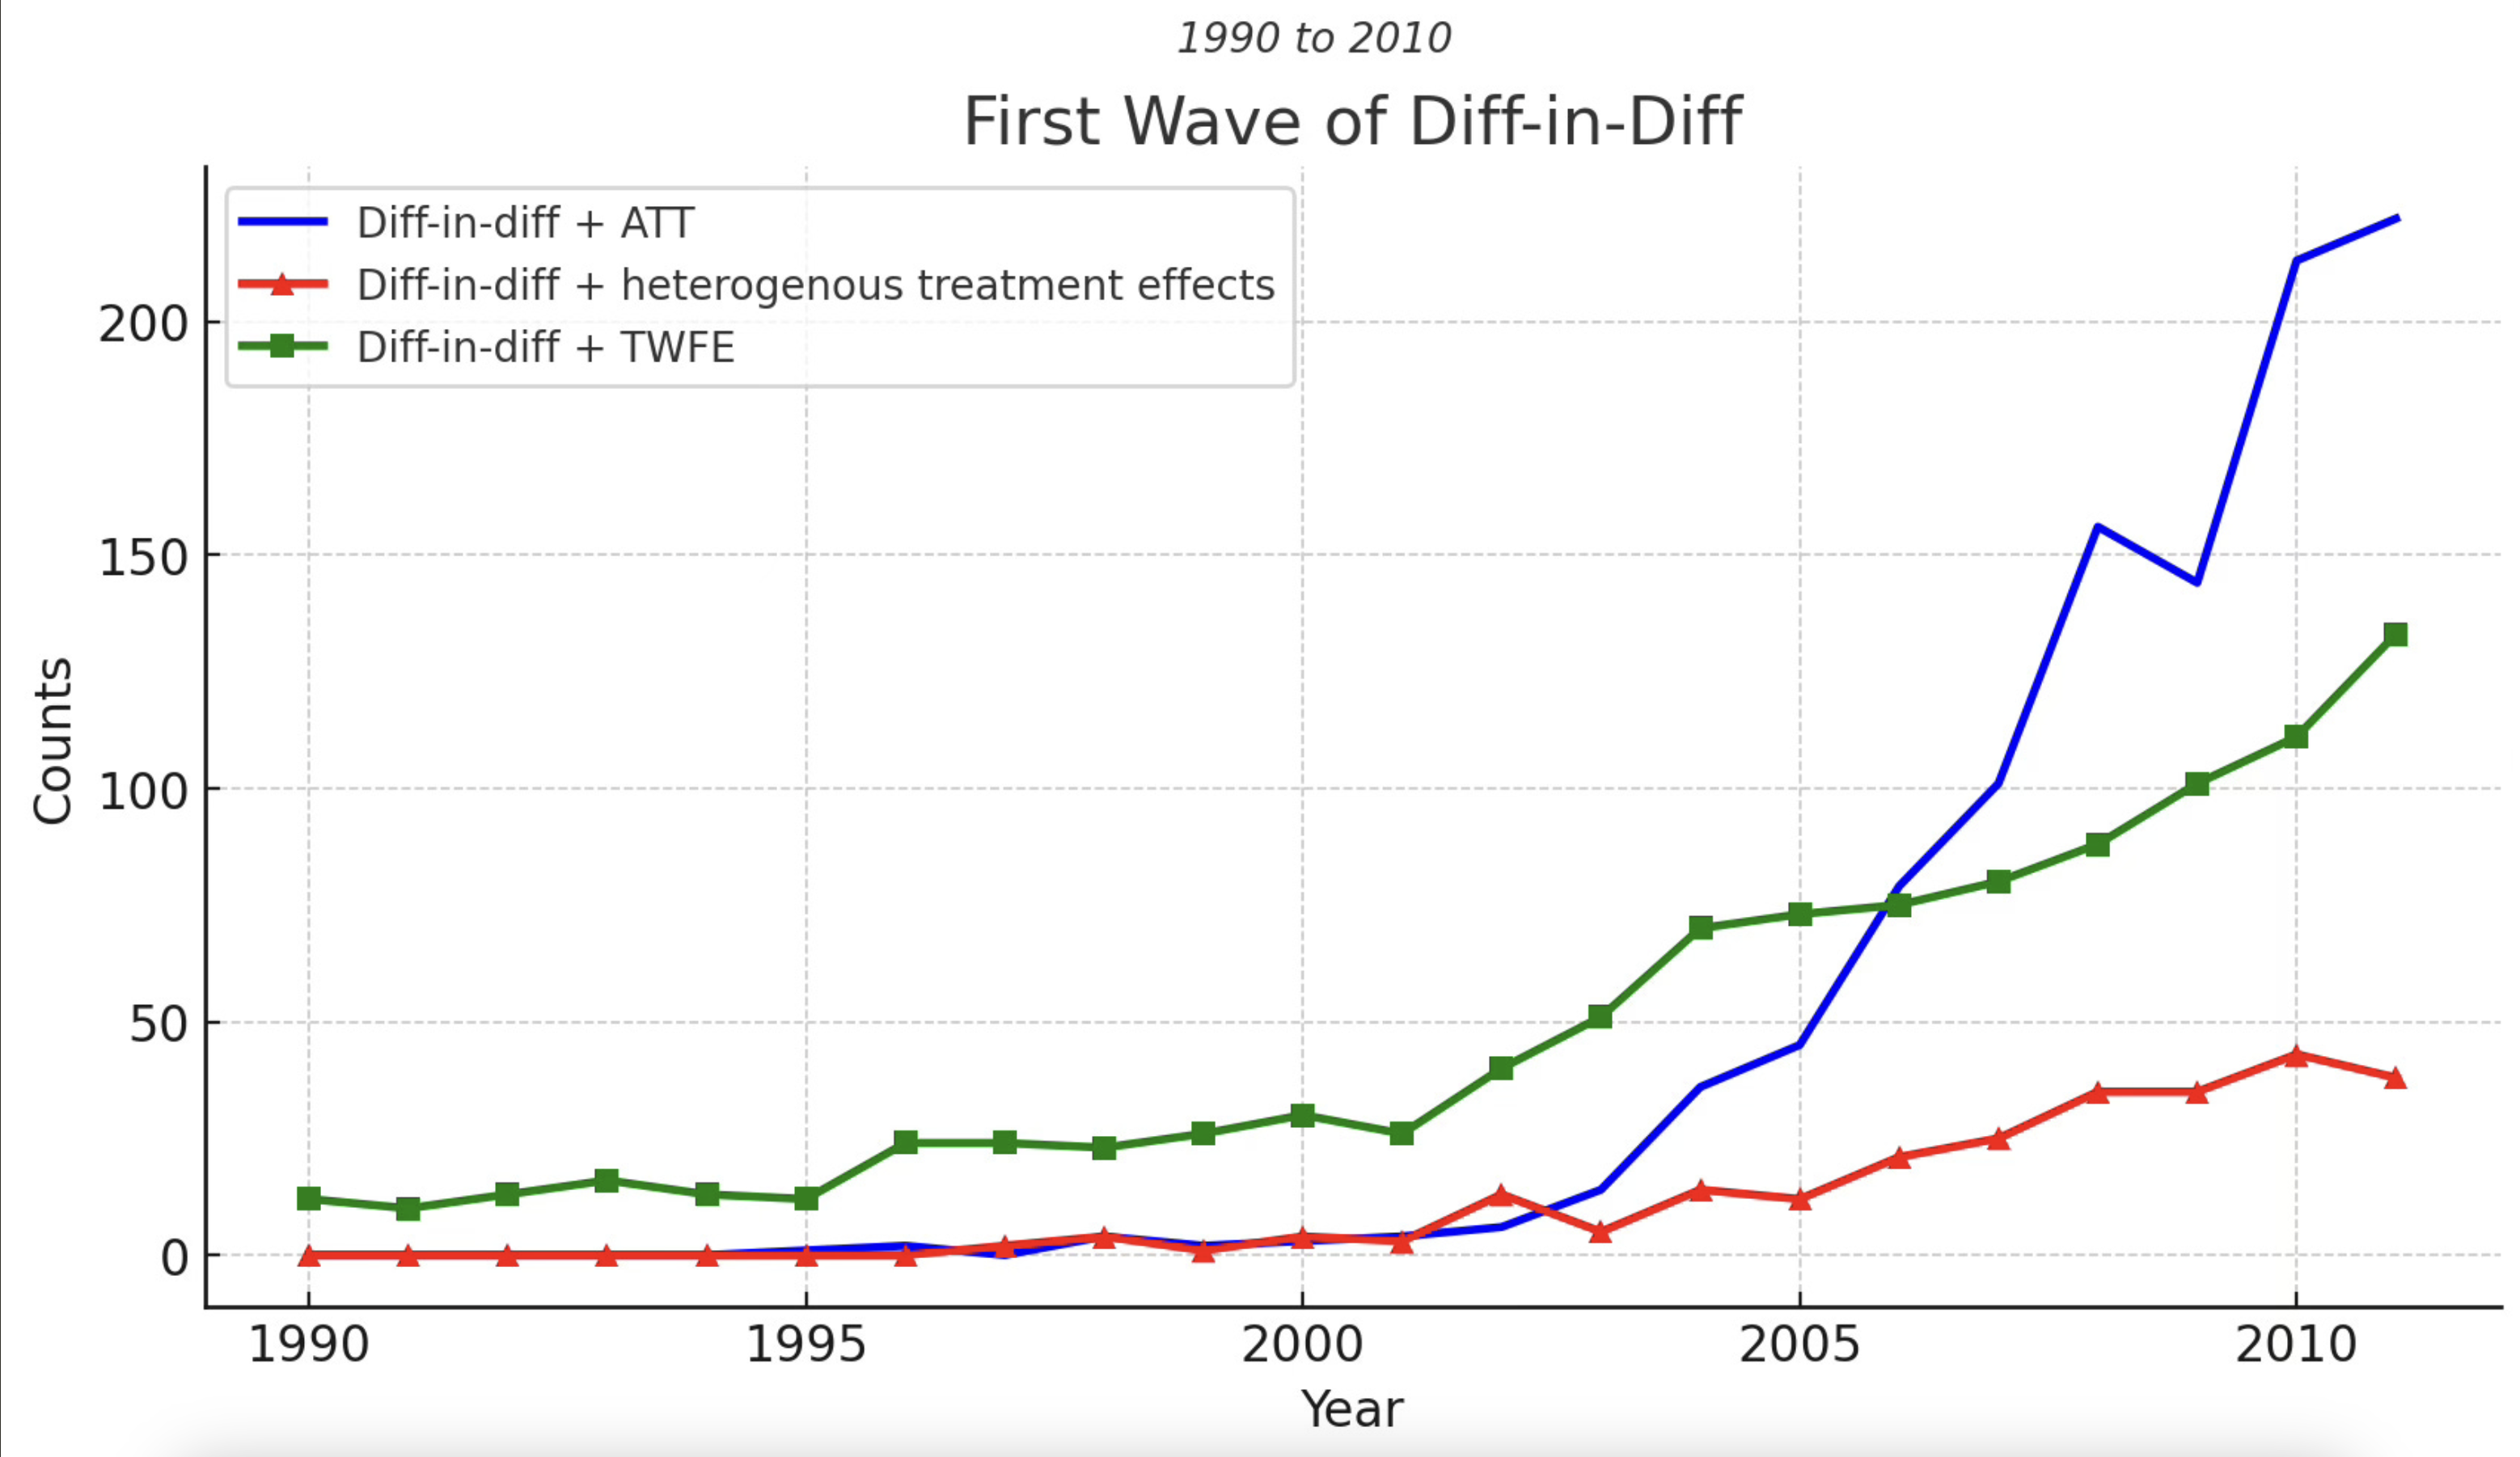
\includegraphics[scale=0.15]{./lecture_includes/wave1}
	\end{figure}

\end{frame}


\begin{frame}{Second Wave}

	\begin{figure}
	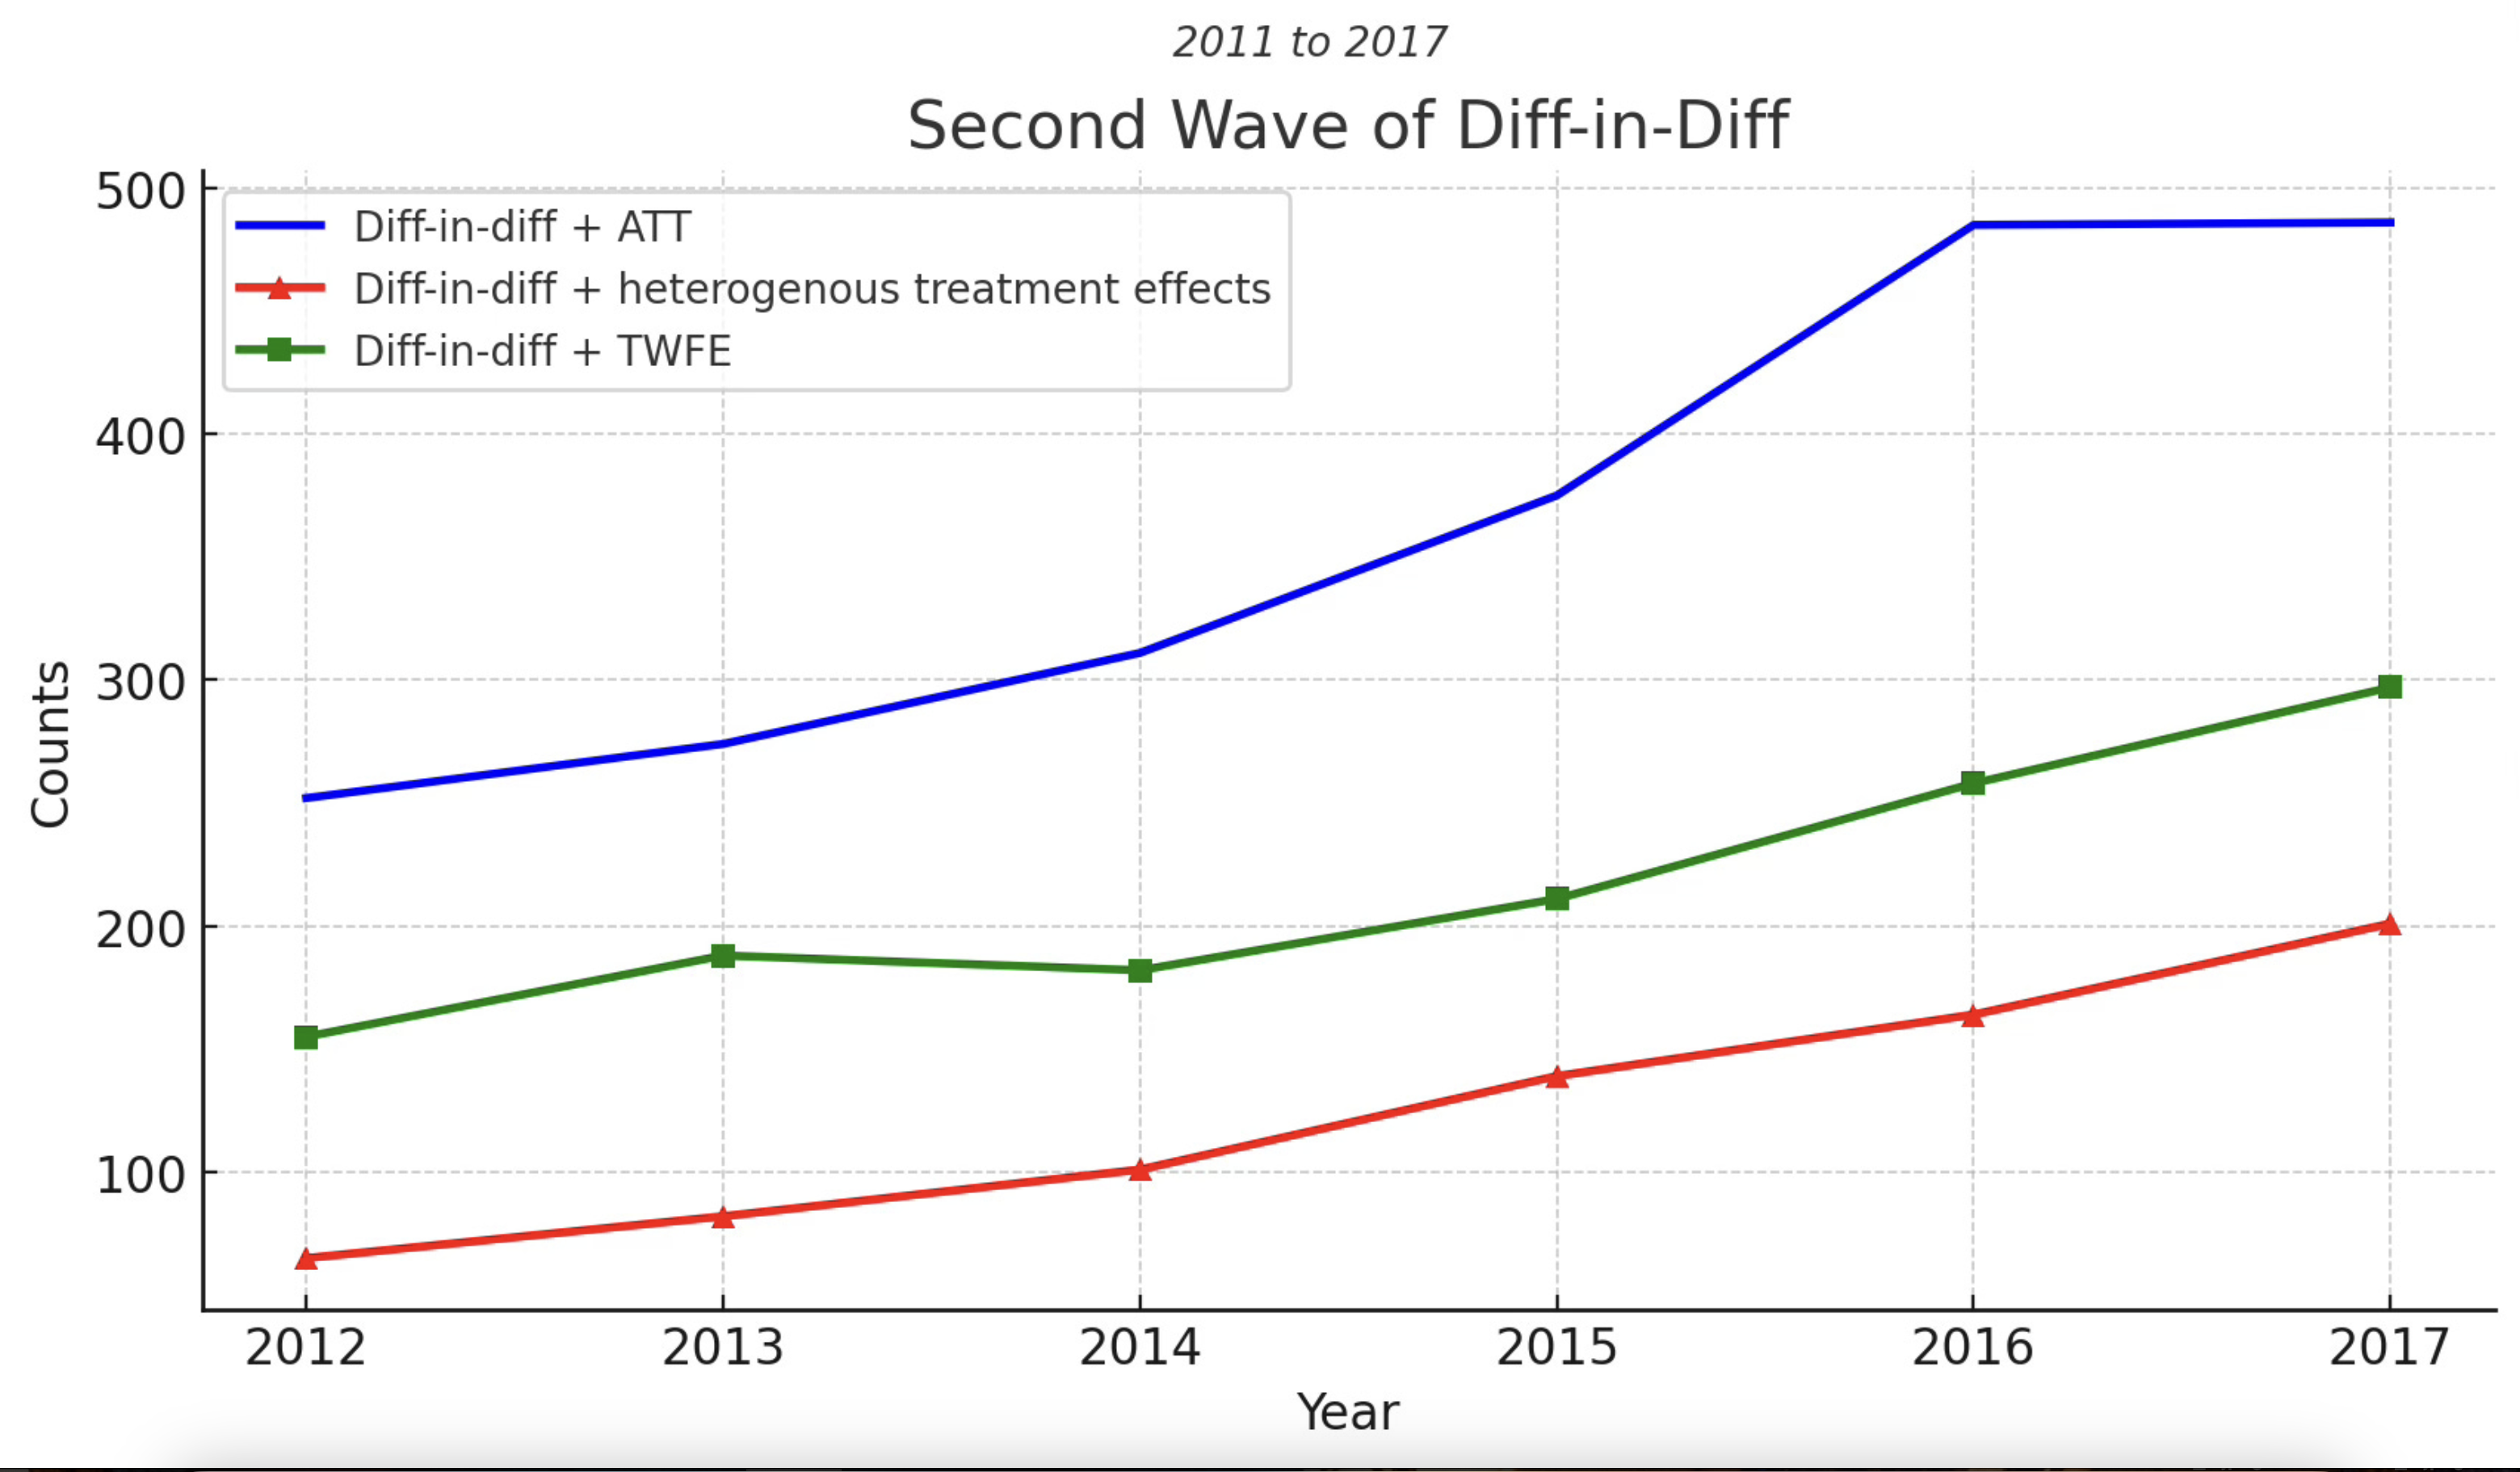
\includegraphics[scale=0.15]{./lecture_includes/wave2}
	\end{figure}

\end{frame}

\begin{frame}{Third Wave}

	\begin{figure}
	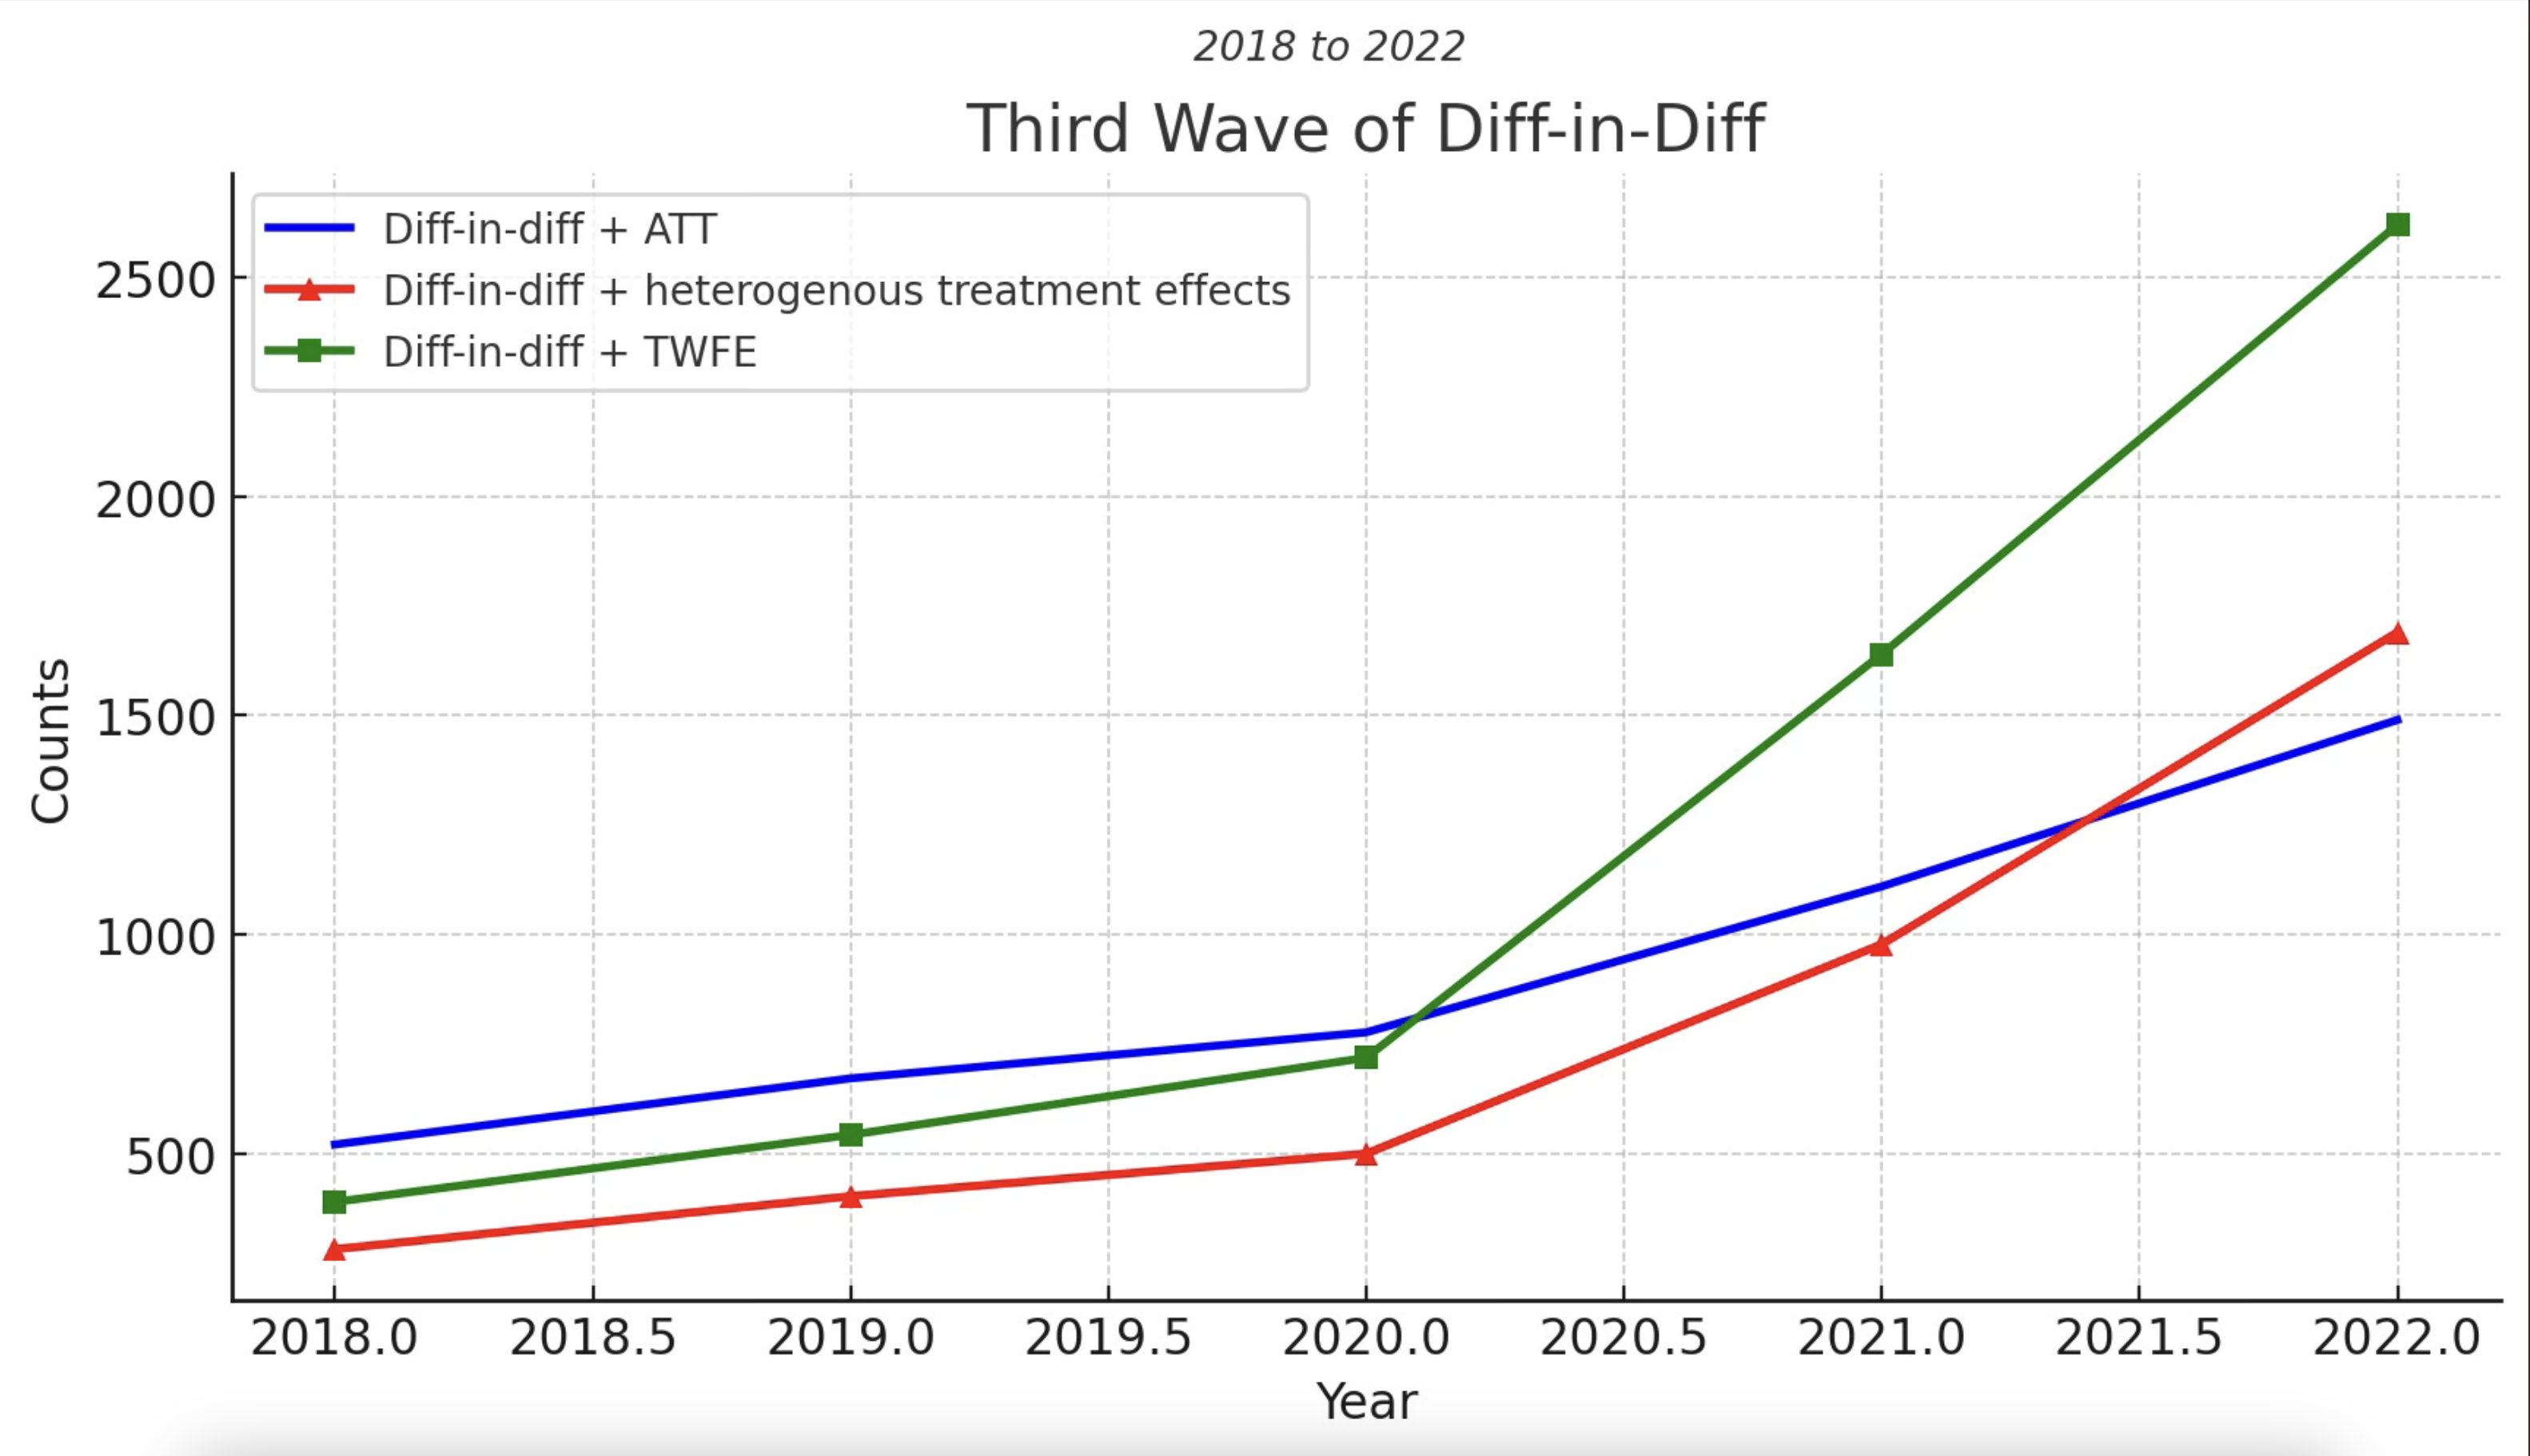
\includegraphics[scale=0.15]{./lecture_includes/wave3}
	\end{figure}

\end{frame}

\begin{frame}{TWFE relative to DID}

	\begin{figure}
	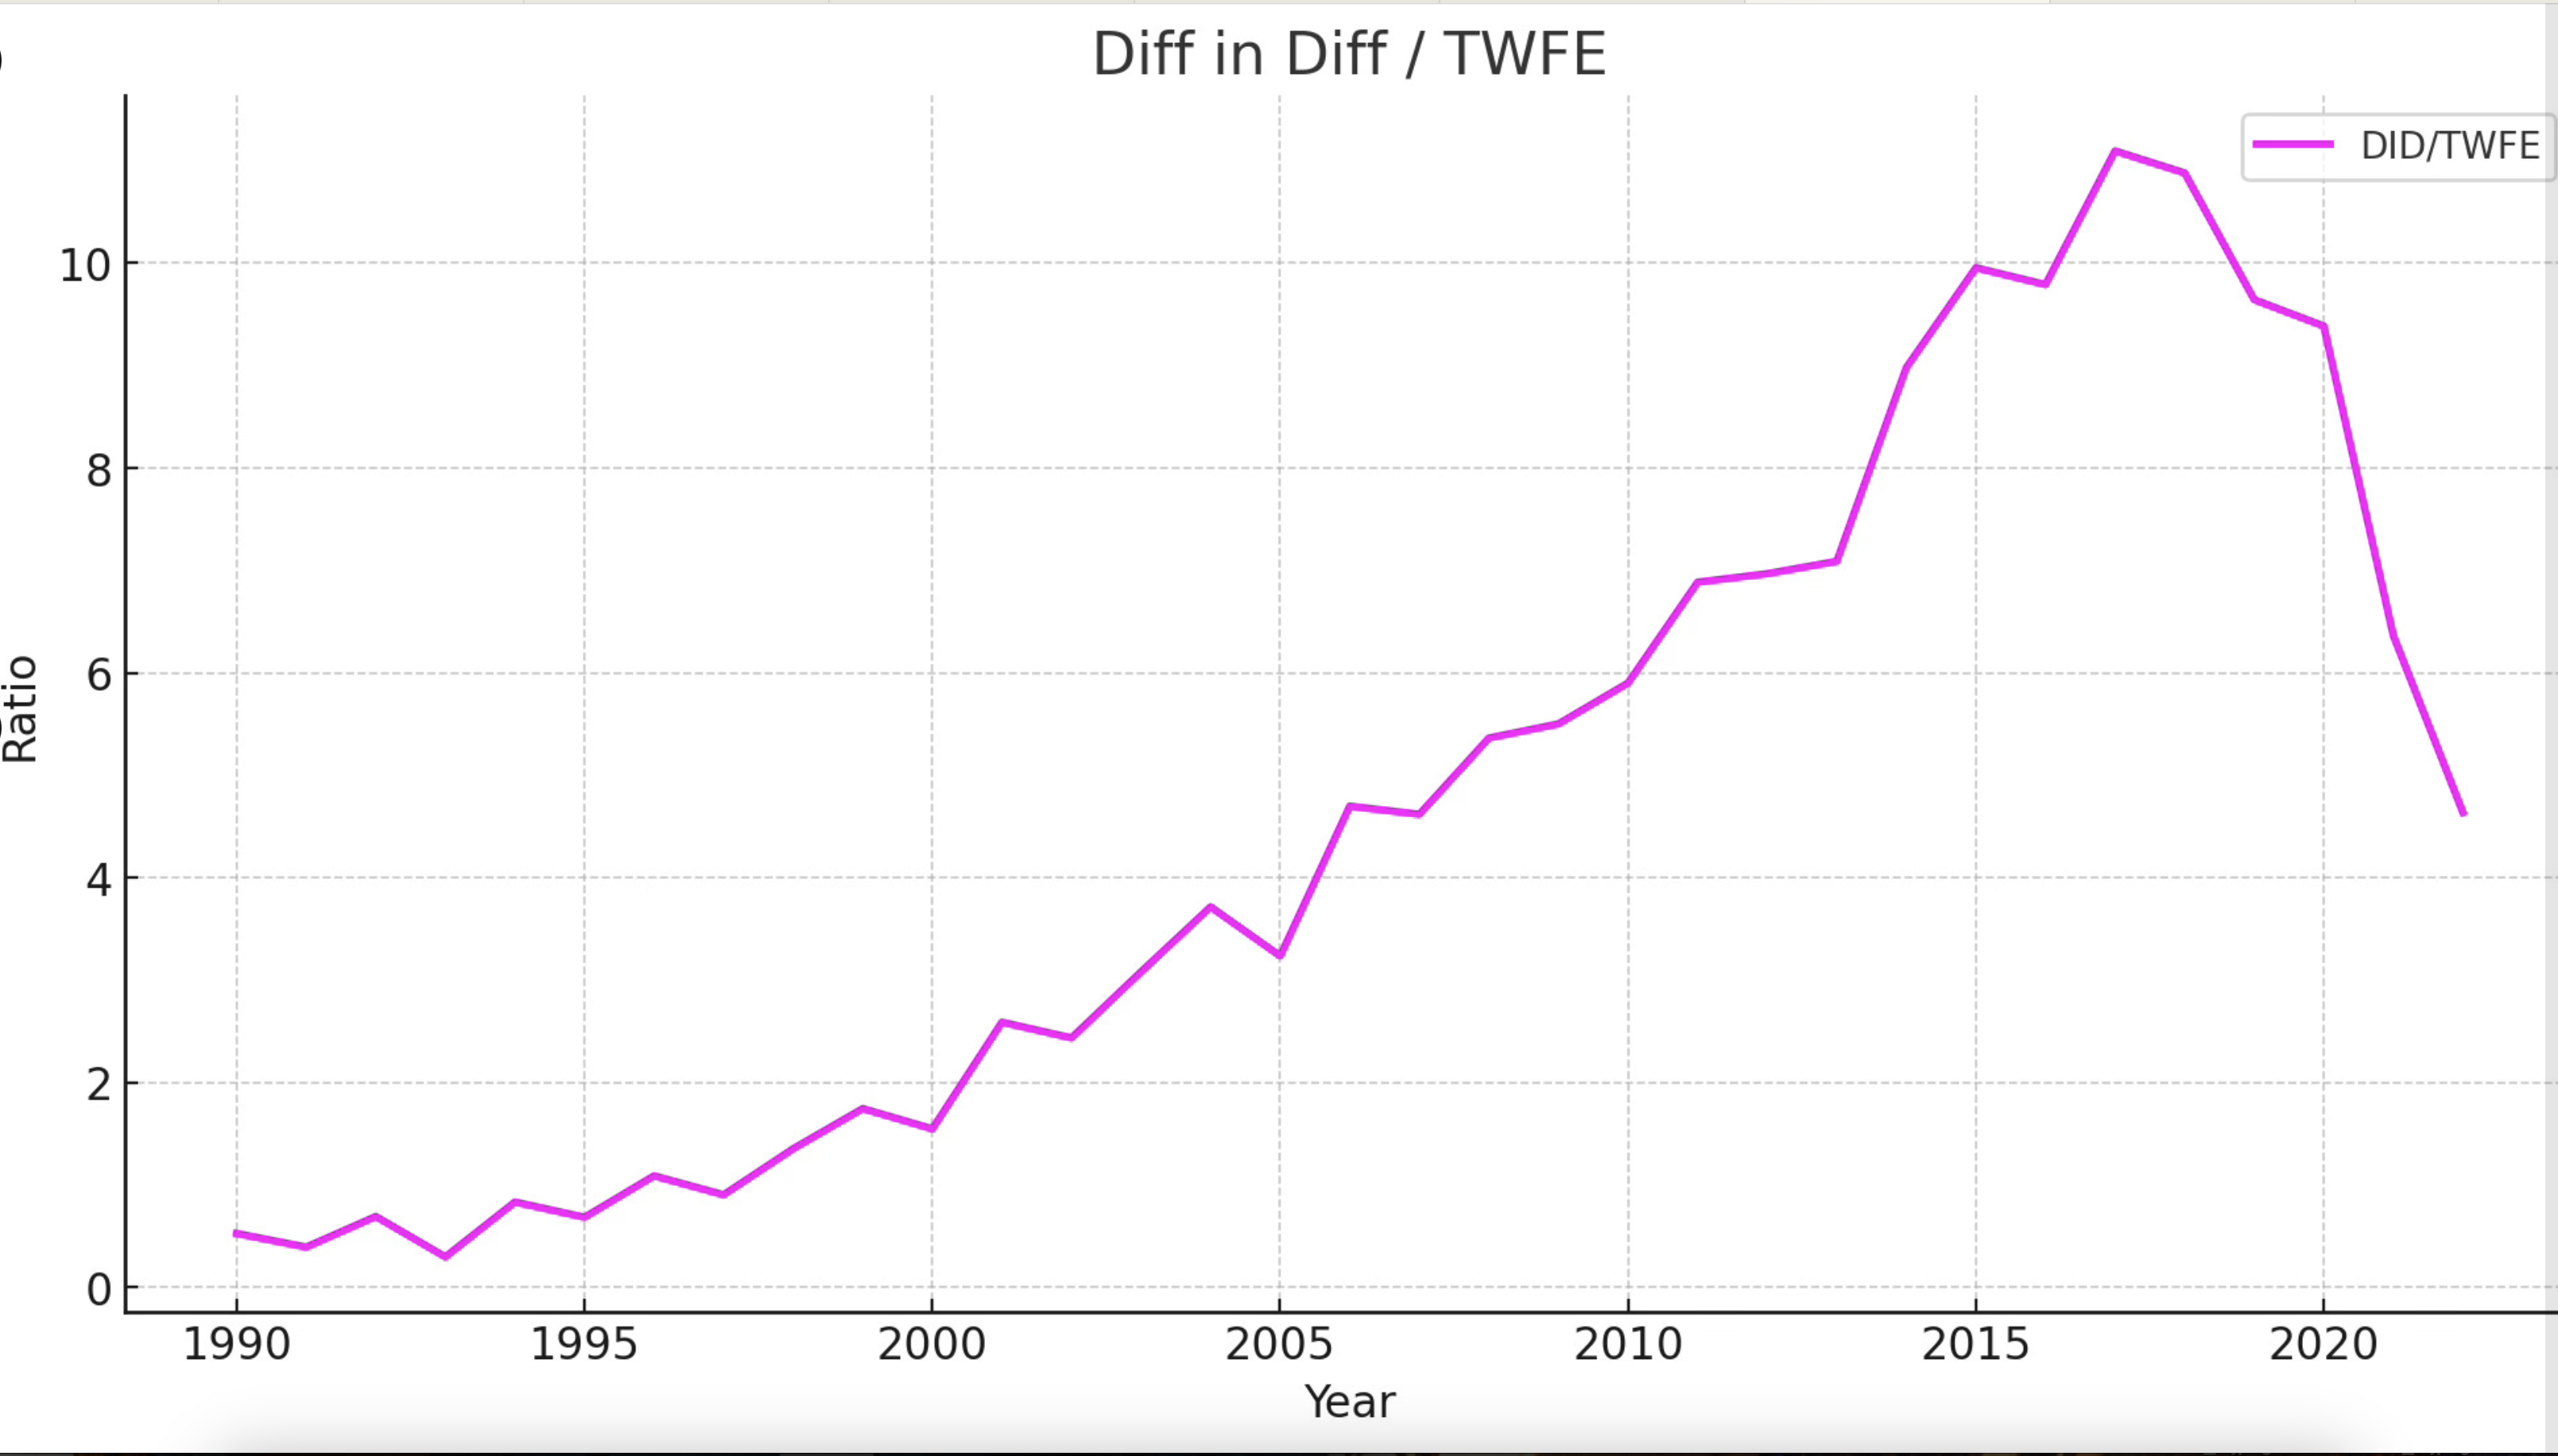
\includegraphics[scale=0.15]{./lecture_includes/wave4}
	\end{figure}

\end{frame}


\begin{frame}{Summarizing the history}

\begin{itemize}

\item Diff-in-diff moves in distinct waves from its simplest forms but does not technically incorporate more contemporary concepts until late in the waves
\item These moves help explain the entire workshop which is largely going to follow those waves
\item And we will be seeing that once the method wraps around potential outcomes, the problems with some models but not others became clear
\item Our focus will be on the parameter of interest, the minimum assumptions needed to identify it, the estimators at our disposal, and what constitutes a convincing case

\end{itemize}

\end{frame}

\section{Difference-in-Differences}


\subsection{Potential outcomes}


\begin{frame}{Traditional econometric steps to any research project}

\begin{enumerate}
\item Convert research question into causal parameter
\item Deduce beliefs needed to estimate that causal parameter with data
\item Create a calculator that will use data and estimate the causal parameter
\end{enumerate}

\bigskip

But many skip (1) and maybe even (2) and instead simply ``run regressions'' and cross our fingers that that coefficient is causal, but is it? And why is it?  And what is it? 

\end{frame}


\begin{frame}{OLS Measures Four Averages and Three Subtractions}
$$Y_{ist} = \alpha_0 + \alpha_1 Treat_{is} + \alpha_2 Post_{t} + \textcolor{blue}{\delta} (Treat_{is} \times Post_t) + \varepsilon_{ist} $$

\bigskip

$$\widehat{\textcolor{blue}{\delta}} = \bigg ( \overline{y}_k^{post(k)} - \overline{y}_k^{pre(k)} \bigg ) - \bigg ( \overline{y}_U^{post(k)} - \overline{y}_U^{pre(k)} \bigg ) $$

\begin{itemize}
\item Orley claims that the OLS estimator of $\delta$ and the ``four averages and three subtractions'' calculation are numerically identical \\ \url{https://youtu.be/WnB3EJ8K7lg?t=126}
\item Review these two calculations using \texttt{equivalence.do} in Stata to illustrate the point
\end{itemize}

\end{frame}

\begin{frame}{Introducing Potential Outcomes to DiD}

\begin{itemize}
\item We want to know when does the DiD equation identify a causal parameter and which one (there are several)?
\item We need causality concepts that can be linked to DiD if we are to answer this question
\item Potential outcomes notation is the main language of modern causal inference and is rooted in the early experimental design writers like Ronald Fisher and Jerzey Neyman, as well as modern statisticians like Don Rubin
\end{itemize}

\end{frame}




\begin{frame}{Potential outcomes notation}
	
	\begin{itemize}
	\item Let the treatment be a binary variable: $$D_{i,t} =\begin{cases} 1 \text{ if in job training program $t$} \\ 0 \text{ if not in job training program at time $t$} \end{cases}$$where $i$ indexes an individual observation, such as a person

	\end{itemize}
\end{frame}

\begin{frame}{Potential outcomes notation}
	
	\begin{itemize}

	\item Potential outcomes: $$Y_{i,t}^j =\begin{cases} 1 \text{: wages at time $t$ if trained} \\ 0 \text{: wages at time $t$ if not trained} \end{cases}$$where $j$ indexes a counterfactual state of the world

	\end{itemize}
\end{frame}



\begin{frame}{Treatment effect definitions}


	\begin{block}{Individual treatment effect}
	    The individual treatment effect,  $\delta_i$, equals $Y_i^1-Y_i^0$
	\end{block}

Missing data problem:  No ones the counterfactual (no matter how confident they are)
	
\end{frame}


\begin{frame}{Conditional Average Treatment Effects}	
	\begin{block}{Average Treatment Effect on the Treated (ATT)}
	The average treatment effect on the treatment group is equal to the average treatment effect conditional on being a treatment group member:
		\begin{eqnarray*}
		E[\delta|D=1]&=&E[Y^1-Y^0|D=1] \nonumber \\
		&=&E[Y^1|D=1]-\textcolor{red}{E[Y^0|D=1]}
		\end{eqnarray*}
	\end{block}
	
	\bigskip

It's the average causal effect but only for the people exposed to some intervention; notice we can't calculate it, also, because we are missing the red term

	
\end{frame}

\begin{frame}{Potential outcomes vs realized data}

\begin{itemize}
\item Potential outcomes are \emph{a priori} real but unknown descriptions of states of the world under different treatment exposures
\item Realized data are selected from the potential outcomes based on one's treatment assignment which we can show using the switching equation
 $$Y_{it}=D_{it}Y_{it}^1 + (1-D_{it})Y_{it}^0$$
\item How those treatment get assigned is called the treatment assignment mechanism

\end{itemize}
\end{frame}

\begin{frame}{Simple spreadsheet exercise}

Let's review basic concepts here at "WEIGHTS" tab: \url{https://docs.google.com/spreadsheets/d/10DuQqGtH_Ewea7zQoLTFYHbnvqaTVDhn2GDzq3Oa6EQ/edit?usp=sharing}

\end{frame}

\subsection{Identification, Estimation and Inference}


\begin{frame}{DiD equation is the 2x2}

Orley's ``four averages and three subtractions'' uses two groups, two time periods, or 2x2

\begin{eqnarray*}
\widehat{\delta} = \bigg ( E[Y_k|Post] - E[Y_k|Pre] \bigg ) - \bigg ( E[Y_U | Post ] - E[ Y_U | Pre] \bigg) \\
\end{eqnarray*}$k$ are the people in the job training program, $U$ are the untreated people not in the program, $Post$ is after the trainees took the class, $Pre$ is the period just before they took the class, and $E[y]$ is mean earnings. 

\bigskip

When will $\widehat{\delta}$ equal the ATT?  When will it not?

\end{frame}



\begin{frame}{Replace with potential outcomes and add a zero}

\begin{eqnarray*}
\widehat{\delta} &=& \bigg ( \underbrace{E[Y^1_k|Post] - E[Y^0_k|Pre] \bigg ) - \bigg ( E[Y^0_U | Post ] - E[ Y^0_U | Pre]}_{\mathclap{\text{Switching equation}}} \bigg)  \\
&&+ \underbrace{\textcolor{red}{E[Y_k^0 |Post] - E[Y^0_k | Post]}}_{\mathclap{\text{Adding zero}}} 
\end{eqnarray*}

\end{frame}

\begin{frame}{Parallel trends bias}

\begin{eqnarray*}
\widehat{\delta} &=& \underbrace{E[Y^1_k | Post] - \textcolor{red}{E[Y^0_k | Post]}}_{\mathclap{\text{ATT}}} \\
&& + \bigg [  \underbrace{\textcolor{red}{E[Y^0_k | Post]} - E[Y^0_k | Pre] \bigg ] - \bigg [ E[Y^0_U | Post] - E[Y_U^0 | Pre] }_{\mathclap{\text{Non-parallel trends bias in 2x2 case}}} \bigg ]
\end{eqnarray*}


\end{frame}

\begin{frame}{Identification through parallel trends}
	

	\begin{block}{Parallel trends}
	Assume two groups, treated and comparison group, then we define parallel trends as:	 $$\textcolor{red}{E(}\textcolor{red}{\Delta Y^0_k)} = E(\Delta Y^0_U)$$
	\end{block}

\textbf{In words}: ``The \textcolor{red}{evolution of earnings for our trainees \emph{had they not trained}} is the same as the evolution of mean earnings for non-trainees''.  

\bigskip

It's in \textcolor{red}{red} because parallel trends is untestable and critically important to estimation of the ATT using any method, OLS or ``four averages and three subtractions''

	

	
\end{frame}


\begin{frame}{What is and is not parallel trends?}

\begin{itemize}
\item Parallel trends does \emph{not} mean treatments were randomly assigned (though random assignment guarantees parallel trends)
\item Parallel trends does \emph{not} require that the groups be similar at baseline on outcomes (though random assignment guarantees that would be)
\item Parallel trends \emph{does} require that the comparison group follows a trend in outcomes that is approximately the same as the counterfactual trend of the treatment group (what would have had happened had the treatment not occurred)
\end{itemize}

\end{frame}



\begin{frame}{Homework \#1}


\begin{eqnarray*}
\widehat{\delta} &=& \bigg ( E[Y_k|Post] - E[Y_k|Pre] \bigg ) - \bigg ( E[Y_U | Post ] - E[ Y_U | Pre] \bigg) \\
\end{eqnarray*}What if the $U$ group had always been treated in both periods? Is parallel trends enough to identify the ATT?

\bigskip

Replace realized outcomes with potential outcomes and rewrite using the ``add zero'' trick we did.  I'll review the answer tomorrow.


\end{frame}











\begin{frame}{Understanding parallel trends through worksheets}

Before we move into regression, let's go through a simple exercise to really pin down these core ideas with simple calculations

\bigskip 

\url{https://docs.google.com/spreadsheets/d/1onabpc14JdrGo6NFv0zCWo-nuWDLLV2L1qNogDT9SBw/edit?usp=sharing}

\end{frame}


\begin{frame}{Three main DiD assumptions}

\begin{itemize}
\item Parallel trends is the most common one and most well known
\item But parallel trends is nested within a bundle of assumptions, and all of them are need for traditional difference-in-differences
\item Other two lesser known assumptions are "No anticipation" (or NA) and Stable Unit Treatment Value Assumption (SUTVA)

\end{itemize}

\end{frame}


\begin{frame}{No Anticipation}

\begin{itemize}
\item ``No anticipation'' simply means that the unit is not treated until it is treated (and that can be violated with rational forward looking agents but not always)
	\begin{itemize}
	\item \textbf{Example 1}: Tomorrow I win the lottery, but don't get paid yet. I decide to buy a new house today. That violates NA
	\item \textbf{Example 2}: Next year, a state lets you drive without a driver license and you know it. But you can't drive without a driver license today.  This satisfies NA.
	\end{itemize}
\item Violations in simple 2x2 where baseline is treated creates problems that I discuss here: \bigskip

 \url{https://causalinf.substack.com/p/difference-in-differences-no-anticipation}
 
 \bigskip
 
 \url{https://causalinf.substack.com/p/mixtape-mailbag-7-what-happens-in}
\end{itemize}

\end{frame}


\begin{frame}{Second homework assignment}


\begin{eqnarray*}
\widehat{\delta} &=& \bigg ( E[Y_k|Post] - E[Y_k|Pre] \bigg ) - \bigg ( E[Y_U | Post ] - E[ Y_U | Pre] \bigg) \\
\end{eqnarray*}What if the $k$ group had been treated at the baseline ``pre'' period in our 2x2?  

\bigskip

Replace realized outcomes with potential outcomes and rewrite using the ``add zero'' trick we did.  I'll review the answer tomorrow, but let's skip to the result here

\end{frame}

\begin{frame}{No Anticipation Violation}

If the baseline period is treated, then the simple 2x2 identifies the following three terms:

\begin{eqnarray*}
\delta &=& ATT_k(Post) \\&&+ \text{Non PT bias} \\&&- ATT_k(Pre)
\end{eqnarray*}

First row is the ATT in the post period; middle row is parallel trends; third row subtracts the baseline ATT from the calculation. If treatment effects are constant, then the DiD coefficient will be zero despite positive treatment effects.  Let's look in \texttt{na.do}.

\end{frame}



\begin{frame}{SUTVA}

\begin{itemize}
\item Stable Unit Treatment Value Assumption (Imbens and Rubin 2015) focuses on what happens when in our analysis we are combining units (versus defining treatment effects)
	\begin{enumerate}
	\item \textbf{No Interference}: a treated unit cannot impact a control unit such that their potential outcomes change (unstable treatment value)
	\item \textbf{No hidden variation in treatment}: When units are indexed to receive a treatment, their dose is the same as someone else with that same index
	\item \textbf{Scale}: If scaling causes interference or changes inputs in production process, then \#1 or \#2 are violated
	\end{enumerate}
\item Shifts from defining treatment effects to estimating them, which means being careful about who is the control group, how you define treatments and what questions can and cannot be answered with this method
\end{itemize}

\end{frame}

\begin{frame}{Setup for SUTVA}

\begin{eqnarray*}
\widehat{\delta}& =& \bigg ( \underbrace{E[Y_k|Post] - E[Y_k|Pre] \bigg ) - \bigg ( E[Y_U | Post ] - E[ Y_U | Pre]}_{\mathclap{\text{Diff-in-diff}}} \bigg) \\ 
&=& \bigg ( \underbrace{E[Y^1_k|Post] - E[Y^0_k|Pre] \bigg ) - \bigg ( E[\textcolor{blue}{Y^0_U} | Post ] - E[ Y^0_U | Pre]}_{\mathclap{\text{Switching equation with SUTVA in blue}}} \bigg)   \\
&&+ \underbrace{\textcolor{red}{E[Y_k^0 |Post] - E[Y^0_k | Post]}}_{\mathclap{\text{Adding zero}}}
\end{eqnarray*}


\end{frame}

\begin{frame}{Illustrate the role of SUTVA}


Rearrange

\begin{eqnarray*}
\widehat{\delta} &=& \underbrace{E[Y^1_k | Post] - \textcolor{red}{E[Y^0_k | Post]}}_{\mathclap{\text{ATT}}} \\
&& + \bigg [  \underbrace{\textcolor{red}{E[Y^0_k | Post]} - E[Y^0_k | Pre] \bigg ] - \bigg [ E[\textcolor{blue}{Y^0_U} | Post] - E[Y_U^0 | Pre] }_{\mathclap{\text{Non-parallel trends bias in 2x2 case}}} \bigg ]
\end{eqnarray*}

\bigskip

Notice how NA and SUTVA are key for making DiD be this simple expression.


\end{frame}

\begin{frame}{Summarizing}

\begin{itemize}

\item Lots of restrictions placed on difference-in-differences
	\begin{itemize}
	\item NA: you chose a baseline that is not treated
	\item SUTVA: your comparison group is never treated during the course of the calculations
	\item PT: your comparison group has a trend in $E[Y^0]$ that is the same as the counterfactual 
	\end{itemize}
\item Only when you have NA and SUTVA does DiD equal ATT + PT
\item But it's crucial to remember: DiD and ATT are not the same thing

\end{itemize}

\end{frame}








\begin{frame}{OLS Specification}
	
	\begin{itemize}
	\item Simple DiD equation will identify ATT under parallel trends
	\item But so will a particular OLS specification (two groups and no covariates)
	\item OLS was historically preferred because
		\begin{itemize}
		\item OLS estimates the ATT under parallel trends
		\item Easy to calculate the standard errors
		\item Easy to include multiple periods
		\end{itemize}
	\item People liked it also because of differential timing, continuous treatments and covariates, but those are more complex so we address them later
	\end{itemize}
\end{frame}

\begin{frame}{Minimum wages}

\begin{itemize}
\item Card and Krueger (1994) have a famous study estimating causal effect of minimum wages on employment
\item  New Jersey raises its minimum wage in April 1992 (between February and November) but neighboring Pennsylvania does not
\item Using DiD, they do not find a negative effect of the minimum wage on employment leading to complex reactions from economists
\item Orley's describes his understanding of people's reaction to the paper.  \\ \url{https://youtu.be/MOtbuRX4eyQ?t=1882}
\end{itemize}

\end{frame}

\begin{frame}
	\begin{figure}
	\includegraphics[scale=0.5]{./lecture_includes/minwage_whore}
	\end{figure}
\end{frame}


\begin{frame}{Reaction to the paper}


Lots of anecdotes in this interview with Card, but here are just two.  First, Card and Krueger received a lot of personal hostility from their peers (1:07 to 1:10)

\bigskip

\url{https://youtu.be/1soLdywFb_Q?si=laAVYf_E2KBZKywG&t=4020}

\bigskip

Later Card says Sherwin Rosen accused them of having an agenda.  But the worst is what happens to Alan Krueger maybe (1:16 to 1:17)

\bigskip

\url{https://youtu.be/1soLdywFb_Q?si=jsb8h50ZosGDnKrv&t=4556}




\end{frame}

\begin{frame}{Card on that study}

\begin{quote}
``I’ve subsequently stayed away from the minimum wage literature for a number of reasons. First, it cost me a lot of friends. People that I had known for many years, for instance, some of the ones I met at my first job at the University of Chicago, became very angry or disappointed. They thought that in publishing our work we were being traitors to the cause of economics as a whole.''
\end{quote}


\end{frame}



\begin{frame}{OLS specification of the DiD equation}
	
	\begin{itemize}
	\item The correctly specified OLS regression is an interaction with time and group fixed effects:$$Y_{its} = \alpha + \gamma NJ_s + \lambda d_t + \delta (NJ \times d)_{st} + \varepsilon_{its}$$
		\begin{itemize}
		\item NJ is a dummy equal to 1 if the observation is from NJ
		\item d is a dummy equal to 1 if the observation is from November (the post period)
		\end{itemize}
	\item This equation takes the following values
		\begin{itemize}
		\item PA Pre: $\alpha$
		\item PA Post: $\alpha + \lambda$
		\item NJ Pre: $\alpha + \gamma$
		\item NJ Post: $\alpha + \gamma + \lambda + \delta$
		\end{itemize}
	\item DiD equation: (NJ Post - NJ Pre) - (PA Post - PA Pre) $= \delta$
	\end{itemize}
\end{frame}




\begin{frame}[plain]
	$$Y_{ist} = \alpha + \gamma NJ_s + \lambda d_t + \delta(NJ\times d)_{st} + \varepsilon_{ist}$$
	\begin{figure}
	\includegraphics[scale=0.90]{./lecture_includes/waldinger_dd_5.pdf}
	\end{figure}
\end{frame}


\begin{frame}[plain]
	$$Y_{ist} = \alpha + \gamma NJ_s + \lambda d_t + \delta(NJ\times d)_{st} + \varepsilon_{ist}$$
	\begin{figure}
	\includegraphics[scale=0.90]{./lecture_includes/waldinger_dd_5.pdf}
	\end{figure}

Notice how OLS is ``imputing'' $E[Y^0|D=1,Post]$ for the treatment group in the post period? It is only ``correct'', though, if parallel trends is a good approximation

\end{frame}


\begin{frame}{Inference in DID}
  When dealing with clustered data, a crucial concept is the difference between correlated observations and correlated errors. While they may seem similar, they are distinct, and it's essential to focus on the errors when clustering standard errors.
\end{frame}

\begin{frame}{Correlated Observations}
  \begin{itemize}
    \item Correlated observations occur when the observed variables themselves are correlated within a cluster.
    \item For instance, incomes within a specific region might be positively correlated.
    \item Correlated observations do not necessarily violate OLS assumptions.
  \end{itemize}
\end{frame}

\begin{frame}{Correlated Errors}
  \begin{itemize}
    \item Correlated errors occur when the unobserved errors are correlated within a cluster.
    \item This violates the assumption of independent errors, leading to possibly biased standard errors and higher over rejection rates
    \item Failing to account for correlated errors can lead to misleading inference.
  \end{itemize}
\end{frame}


\begin{frame}{Serial correlation creates problems}
  \begin{itemize}
	\item  Bertrand, Duflo and Mullainathan (2004) show that conventional standard errors will often severely understate the standard deviation of the estimators
	\item They proposed three solutions, but most only use one of them (clustering)
	    \item Clustering standard errors accounts for this within-cluster correlation and is a more conservative approach 
	    \item Clustering is typically recommended at the aggregate unit where the entire treatment occurred

  \end{itemize}
\end{frame}






%\begin{frame}{Computing Cluster-Robust Standard Errors}
%  \begin{enumerate}
%    \item Run your regression to get \( u \) and \( \hat{Y} \).
%    \item Calculate cluster-level residuals \( \hat{u}_c \).
%    \item Calculate the "meat" (as in bread-meat-bread sandwich) \( M \) as \( \sum_c X_c^\prime \hat{u}_c \hat{u}_c^\prime X_c \).
%    \item Your standard error covariance matrix is \( \hat{V} = (X^\prime X)^{-1} M (X^\prime X)^{-1} \).
%  \end{enumerate}
  
%  \bigskip
  
%  Mixtape reference (chapter 2): \url{https://mixtape.scunning.com/02-probability\_and\_regression\#cluster-robust-standard-errors}
%\end{frame}

%\begin{frame}{Compressing Into a Single Number}
%  \begin{itemize}
%    \item Diagonal elements of \( \hat{V} \) contain variances for each coefficient.
%    \item Standard errors are the square root of these diagonal elements.
%    \item Non-diagonal elements are used for hypothesis tests and confidence intervals for combinations of coefficients.
%  \end{itemize}
%\end{frame}





\section{Parallel Trends Violations}

\subsection{Results versus Evidence}

\begin{frame}{Court metaphor}

	\begin{itemize}
	\item Think a prosecutor arguing against a defense attorney to convince a judge and jury
	\item The claim the defendant is guilty but the claim is not the evidence -- it's more like an assertion
	\item The evidence is the smoking gun, the fingerprints, the eye witnesses, the footprints in the mud outside the house
	\item If your claim is supported by weak evidence, then no one \emph{should} convict -- it would be borderline corruption if they did 
	\end{itemize}

\end{frame}


\begin{frame}{Evidence versus the Main Result}

\begin{itemize}
\item Causal inference is about \emph{warranted beliefs} -- should you or should you not believe the \emph{causal claim}?
\item Your DiD \emph{results} are like the claim of guilt, but your DiD results are \emph{not} the smoking gun
\item You need to provide evidence for parallel trends against several well known vulnerabilities
\item Evidence will be bite, falsifications, mechanisms and event study data visualization 
\item We will mix the parallel trends violations with the evidence concept before getting into advanced estimators
\end{itemize}

\end{frame}





\begin{frame}{Three classic parallel trends violations}

	\begin{enumerate}
	\item Compositional change with repeated cross-sections
	\item Policy endogeneity
	\item Covariates
	\end{enumerate}
\bigskip



\end{frame}

\subsection{Compositional Changes and Cross Sections}



\begin{frame}{Repeated cross-sections and compositional change}
	
	\begin{itemize}
	\item One of the risks of a repeated cross-section is that the composition of the sample may have changed between the pre and post period in ways that are correlated with treatment
	\item Hong (2013) uses repeated cross-sectional data from the Consumer Expenditure Survey (CEX) containing music expenditure and internet use for a random sample of households
	\item Study exploits the emergence of Napster (first file sharing software widely used by Internet users) in June 1999 as a natural experiment
	\item Study compares internet users and internet non-users before and after emergence of Napster
	\end{itemize}

\end{frame}

\begin{frame}{Introduction of Napster and spending on music}
	\begin{figure}
	\includegraphics[scale=0.5]{./lecture_includes/hong_napster}
	\end{figure}
	
\end{frame}


\begin{frame}[plain]
	\begin{figure}
	\includegraphics{./lecture_includes/Hong_1.pdf}
	\end{figure}
	
\end{frame}





\begin{frame}[shrink=20,plain]
	\begin{figure}
	\includegraphics{./lecture_includes/Hong_2.pdf}
	\end{figure}
	
	Diffusion of the Internet changes samples (e.g., younger music fans are early adopters)
	
\end{frame}

\begin{frame}{Repeated cross-sections}

\begin{itemize}
\item Surprisingly underappreciated problem with almost no literature around it
\item Replace the outcome with your time-varying covariates and estimate your DiD model
\item Use covariates highly predictive of the missing $E[Y^0|D=1]$ for this exercise
\item ``Difference-in-differences with Compositional Changes'' by Pedro Sant'Anna and Qi Xu is an update to Hong (2013)
\end{itemize}

\end{frame}


\subsection{Event Studies}



\begin{frame}{Event studies have become mandatory in DiD}

	\begin{figure}
	\includegraphics[scale=0.5]{./lecture_includes/currie_eventstudy.png}
	\end{figure}

\end{frame}

\begin{frame}{Intuition behind event studies}

\begin{itemize}

	\item We cannot directly verify parallel trends, so for a long time researchers have focused on the pre-trends (Ashenfelter's Dip)
	\item Parallel pre-trends not required for parallel trends and vice versa, but this is the smoking gun we typically look for nonetheless
	\item Think of it as a type of check for selection bias, but imperfect with false positives and false negatives
	\item Even if pre-trends are the same one still has to worry about other policies changing at the same time (omitted variable bias is a parallel trends violation)

\end{itemize}

\end{frame}



\begin{frame}{Creating event studies}

\begin{itemize}

\item Originally, there were no event studies (as we saw in the First Wave)
\item Economists pulled from finance and took the event study concept and changed it to suit Ashenfelter Dip reasoning
\item Always presented graphically, but there were different ways people went about it so we will review them and make suggestions

\end{itemize}

\end{frame}



\begin{frame}{Plot the raw data when there's only two groups}

	\begin{figure}
	\includegraphics[scale=2.5]{./lecture_includes/waldinger_dd_6.pdf}
	\end{figure}

\end{frame}


\begin{frame}{Event study regression}
	
	\begin{itemize}
	\item Alternatively, present estimated coefficients from a dynamic regression specification:
 $$Y_{its} = \alpha + \sum_{\tau=-2}^{-q}\mu_{\tau} (D_s \times \tau_t) + \sum_{\tau=0}^m\delta_{\tau} (D_s \times \tau_t) + \tau_t + D_s + \varepsilon_{ist}$$
		\begin{itemize}
		\item With a simple 2x2, you are interacting treatment indicator with calendar year dummies
		\item Includes $q$ leads or anticipatory effects and $m$ lags or post treatment effects
		\end{itemize}
	\item Estimated $\widehat{\delta}$ coefficients are estimated ATT parameters assuming parallel trends and $\widehat{\mu}$ is part of your evidence for that
	\end{itemize}
\end{frame}

\begin{frame}{Event study regression}


\begin{itemize}
\item  Typically you'll plot the coefficients and 95\% CI on all leads and lags (binned or not, trimmed or not) 
\item Under No Anticipation, SUTVA and parallel pre-trends, then mechanically $\widehat{\mu_{\tau}}$ will be zero (does not guarantee the same about post-trends)
\item There are still specification and power issues that Jon Roth has written about, but I will skip that
\item But also under NA, SUTVA and parallel trends (post trends), then $\widehat{\delta}$ are estimates of the ATT at points in time
\end{itemize}

\end{frame}

\begin{frame}{Normal DiD coefficient}

\begin{eqnarray*}
\widehat{\delta} &=& \underbrace{E[Y^1_k | Post] - \textcolor{red}{E[Y^0_k | Post]}}_{\mathclap{\text{ATT}}} \\
&& + \bigg [  \underbrace{\textcolor{red}{E[Y^0_k | Post]} - E[Y^0_k | Pre] \bigg ] - \bigg [ E[Y^0_U | Post] - E[Y_U^0 | Pre] }_{\mathclap{\text{Non-parallel trends bias in 2x2 case}}} \bigg ]
\end{eqnarray*}

\bigskip

But this was \emph{post}-treatment.  Still, put that aside -- diff-in-diff equations \emph{always} identify the sum of those terms, even in the pre-period


\end{frame}

\begin{frame}{Pre-treatment DiD coefficient}

\begin{eqnarray*}
\widehat{\delta}_{t-2} &=& \bigg [  \underbrace{\textcolor{black}{E[Y^0_k | t-2]} - E[Y^0_k | t-1] \bigg ] - \bigg [ E[Y^0_U | t-2] - E[Y_U^0 | t-1] }_{\mathclap{\text{Non-parallel trends bias in 2x2 case}}} \bigg ]
\end{eqnarray*}

\bigskip

Under NA, then the $t-1$ period is untreated.  But then so are the other pre-periods so the ATT is implicitly zero and the \emph{only} thing that you can be measuring with pre-trend DiD coefficients is differential trends.  


\end{frame}



\begin{frame}{Event study coefficients}

\begin{itemize}
\item Remember that the OLS specification we discuss collapses to ATT plus parallel trends bias
\item This is \emph{always} true because it's an identity and holds even in the pre-period as much in the post
\item It's just in the pre period, you do not have the missing $E[Y^0|D=1]$ term as no one and nothing is treated in pre-period under NA
\item This means pre-period is basically an opportunity to directly verify parallel pre-trends -- but it's the past's pre-trends, not the counterfactual pre-trend of the present/future
\item And that's how people use the pre-period -- they use the pre-period to evaluate whether they think this is a good control group
\end{itemize}

\end{frame}

\begin{frame}{Event study example}

\begin{itemize}
\item The notion is really simple: if PT held then, you'll argue that it's reasonable it would've still held
\item But this is an assertion, and you need to build the case as we said
\item At this point, it's a lot easier to show you what I'm talking about -- where the art and the science meet -- with a great paper
\end{itemize}

\end{frame}




\begin{frame}{Medicaid and Affordable Care Act example}

\begin{figure}
\includegraphics[scale=0.25]{./lecture_includes/medicaid_qje}
\end{figure}

\end{frame}
\begin{frame}{Their Evidence versus Their Result}

\begin{itemize}
\item \textbf{Bite} -- they will show that the expansion shifted people into Medicaid and out of uninsured status
\item \textcolor{black}{\textbf{Placebos}} -- they show that there's no effect of Medicaid on a similar group that didn't enroll
\item \textbf{Event study} -- they will lean hard on those dynamic plots
\item \textcolor{red}{\textbf{Main results}} -- with all of this, they will show Medicaid expansion caused near elderly mortality to fall
\item \textcolor{black}{\textbf{Mechanisms}} -- they think they can show it's coming from people treating diseases causing mortality declines to compound over time
\end{itemize}

\end{frame}

\begin{frame}{Bite}

\begin{itemize}
\item Bite is a labor economist's phrase, often used with the minimum wage, to say that the minimum wage actually was binding in the first place
\item Here it means when US states made Medicaid more generous, people got on Medicaid who would not have been on it otherwise
\item And as a bonus, would not have been insured at all without it
\item Not the most exciting result, but imagine if the main results on mortality were shown but there was no evidence for bite -- is it believable?
\end{itemize}

\end{frame}


\imageframe{./lecture_includes/Miller_Medicaid1.png}

\imageframe{./lecture_includes/Miller_Medicaid2.png}

\imageframe{./lecture_includes/Miller_Medicaid3.png}


\begin{frame}{Falsification}

\begin{itemize}

\item Their study focuses on ``near elderly'', which means just under 65
\item They choose just under 65 because in the US, 65 and older are eligible for Medicare so more generous Medicaid is irrelevant
\item \emph{But} probably the near elderly and the elderly are equally susceptible to unobserved factors correlated with the treatment
\item So they painstakingly examine the effects on elderly as a falsification as this will strengthen the parallel trends assumption on the near elderly
\end{itemize}

\end{frame}

\begin{frame}{Falsifications on elderly}

	\begin{figure}
\includegraphics[scale=0.425]{./lecture_includes/placebo_medicaid}
	\end{figure}

\end{frame}

\begin{frame}{Main result}

\begin{itemize}

\item Finally they focus on the main result -- and there's more in the paper than I'm showing
\item Event study plots with same specification as the rest allowing us to look at the pre-trends and the post-treatment coefficients
\item If parallel trends holds, then the post-treatment coefficients are interpreted as ATT parameter estimates for each time period
\item The result alone isn't nearly as strong the result in combination with the rest, but it could still be wrong as parallel trends is ultimately not verfiable
\end{itemize}

\end{frame}



\begin{frame}{Near elderly mortality and Medicaid expansion}

	\begin{figure}
	\includegraphics[scale=0.3]{./lecture_includes/Miller_Medicaid4.png}
	\end{figure}

\end{frame}

\begin{frame}{Summarizing evidence and results}

\begin{itemize}
\item \textbf{Bite}: Increases in enrollment and reductions in uninsured support that there is adoption of the treatment
\item \textbf{Event studies}: Compelling graphics showing similarities between treatment and control
\item \textbf{Falsifications}: no effect on a similar group who isn't eligible
\item \textcolor{red}{Main results}: 9.2\% reduction in mortality among the near-elderly
\item \textcolor{red}{Mechanism}: ``The effect is driven by a reduction in disease-related deaths and grows over time.''
\end{itemize}

\end{frame}

\begin{frame}{Making event study}

\begin{itemize}
\item When there is only one treatment group and one comparison group, then you run a regression with an interaction of the treatment group dummy and the calendar year dummies (plus both separately)
\item You must drop $t-\tau$ as the baseline (e.g., $t-1$) and it must be $Y^0$ untreated comparisons (No Anticipation)
\item I have included in a do file that will do it for you either manually or using coefplot in \texttt{simple\_eventstudy.do} at the shared github labs directory
\end{itemize}

\end{frame}


\begin{frame}{Manually creating the event study}

	\begin{figure}
	\includegraphics[scale=0.20]{./lecture_includes/simple_eventstudy_manual}
	\end{figure}

\end{frame}




\begin{frame}{Creating the event study with Ben Jann's \texttt{coefplot}}

	\begin{figure}
	\includegraphics[scale=0.20]{./lecture_includes/simple_eventstudy.png}
	\end{figure}

\end{frame}





\subsection{Triple differences}




\begin{frame}{Biased diff-in-diff}

\begin{itemize}

\item Many people equate triple differences with falsification exercise, but actually it isn't that -- it is it's own design
\item You use triple differences when diff-if-diff is biased
\item It's used, in other words, when you have a parallel trends violation
\item Miller, Johnson and Wherry (2021) didn't use it because they didn't think they had a parallel trends violation -- so instead they used falsification
\end{itemize}

\end{frame}






\begin{frame}{Biased diff-in-diff \#1}

\begin{table}\centering
\scriptsize
		\caption{Biased diff-in-diff \#1: comparing states}
		\begin{center}
		\begin{tabular}{lll|lc}
		\toprule
		\multicolumn{1}{l}{\textbf{States}}&
		\multicolumn{1}{c}{\textbf{Period}}&
		\multicolumn{1}{c}{\textbf{Outcomes}}&
		\multicolumn{1}{c}{$D_1$}&
		\multicolumn{1}{c}{$D_2$}\\
		\midrule
		Experimental states & Before & $Y=NJ$ \\
		& After & $Y=NJ + NJ_t + D$ & $\textcolor{red}{NJ_t}+D$\\
		\midrule
		& & & & $D + (\textcolor{red}{NJ_t}- PA_t)$ \\
		\midrule
		Non-experimental  & Before & $Y=PA$ \\
		states& After & $Y=PA + PA_t$ & $PA_t$\\
		\bottomrule
		\end{tabular}
		\end{center}
	\end{table}

\begin{eqnarray*}
\widehat{\delta}^{true}_{did} = D + (\textcolor{red}{NJ_t}- PA_t)
\end{eqnarray*}The ATT is D. Assume, though, that parallel trends does not hold, $(\textcolor{red}{NJ_t} \neq PA_t)$

\end{frame}


\begin{frame}{Biased Placebo diff-in-diff}

\begin{table}\centering
\scriptsize
		\caption{Biased placebo diff-in-diff: comparing states but single men and older women}
		\begin{center}
		\begin{tabular}{lll|lc}
		\toprule
		\multicolumn{1}{l}{\textbf{States}}&
		\multicolumn{1}{c}{\textbf{Period}}&
		\multicolumn{1}{c}{\textbf{Outcomes}}&
		\multicolumn{1}{c}{$D_1$}&
		\multicolumn{1}{c}{$D_2$}\\
		\midrule
		Experimental states & Before & $Y=NJ$ \\
		& After & $Y=NJ + NJ_t $ & $\textcolor{red}{NJ_t}$\\
		\midrule
		& & & & $ (\textcolor{red}{NJ_t}- PA_t)$ \\
		\midrule
		Non-experimental  & Before & $Y=PA$ \\
		states& After & $Y=PA + PA_t$ & $PA_t$\\
		\bottomrule
		\end{tabular}
		\end{center}
	\end{table}

\begin{eqnarray*}
\widehat{\delta}^{placebo}_{did} = (\textcolor{red}{NJ_t}- PA_t)
\end{eqnarray*}Assume that parallel trends does not hold, $(\textcolor{red}{NJ_t} \neq PA_t)$

\end{frame}


\begin{frame}{Two biased diff-in-diffs}

\begin{itemize}


\item Parallel trends does not hold, $(\textcolor{red}{NJ_t} \neq PA_t)$, but what if that's the same bias in our placebo DiD?
\item Then we can subtract the second from the first: $$ \widehat{\delta}_{ddd} = \widehat{\delta}^{true}_{did} - \widehat{\delta}^{placebo}_{did}$$
\item Triple differences is a ``real design'' with one parallel trends assumption: $$(\textcolor{red}{NJ_t}^{true}- PA_t^{true}) = (\textcolor{red}{NJ_t}^{placebo}- PA_t^{placebo})$$

\end{itemize}

\end{frame}

\begin{frame}{Triple differences by Gruber (1995)}
	
	\begin{figure}
	\includegraphics{./lecture_includes/gruber_ddd_3.pdf}
	\end{figure}
	
\end{frame}

\begin{frame}{Triple differences commentary}

\begin{itemize}
\item Some people think that it requires that the placebo DiD be zero, but that's incorrect

\item In Gruber's 1995 article, it isn't clear why he needed triple differences in the first place -- his triple differences yielded -0.054 which is almost the same as what he found with his first diff-in-diff (-0.062)
\item The main value of triple differences is that you use it when you believe the parallel trends assumption doesn't hold

\end{itemize}

\end{frame}


\begin{frame}[shrink=20]

\begin{table}\centering
		\caption{Difference-in-Difference-in-Differences (Gruber version)}
		\tiny
		\begin{center}
		\begin{tabular}{lll|l|lll}
		\toprule
		\multicolumn{1}{l}{\textbf{Groups}}&
		\multicolumn{1}{c}{\textbf{States}}&
		\multicolumn{1}{c}{\textbf{Period}}&
		\multicolumn{1}{c}{\textbf{Outcomes}}&
		\multicolumn{1}{c}{$D_1$}&
		\multicolumn{1}{c}{$D_2$}&
		\multicolumn{1}{c}{$D_3$}\\
		\midrule
		&&After	&$NJ+MW+\textcolor{blue}{NJ_t}+\textcolor{red}{MW_t}+D$					\\
	&Experimental			&&&$\textcolor{blue}{NJ_t}+MW_t + D$			\\
		&states&Before	&$NJ+MW$					\\
Married women 					&&&&&$D+\textcolor{blue}{NJ_t} -PA_t 	$	\\
20-40							&&&&&$$\\
    		&&After	&$PA+MW+PA_t+MW_t$					\\
	&Non-experimental		&&	&$PA_t+MW_t$				\\
		&states&Before	&$PA+MW$					\\
								\\
&&&&&&$\textcolor{black}{D}$
\\
		&&After	&$NJ+SO+NJ_t+SO_t$				\\
	&Experimental 			&&&$NJ_t+SO_t$ \\				
		&states&Before	&$NJ+SO$					\\
Single men 					&&&&&$NJ_t  - PA_t$		\\
Older women					&&&&&$$		\\
	     	&&After	&$PA+SO+PA_t+SO_t$					\\
	&Non-experimental		&&&	$PA_t+SO_t$				\\
		&states&Before	&$PA+SO$					\\
		\bottomrule
		\end{tabular}
		\end{center}
	\end{table}

\begin{center}
\textbf{Triple diff assumption}
\end{center}

$\widehat{\delta}_{DDD}= D + \underbrace{[(\textcolor{blue}{NJ^{MW}_t} - PA^{MW}_t) -( NJ^{SO}_t - PA^{SO}_t )]}_{\mathclap{\text{Equally biased  DiD \#1 and \# 2}}}$

\bigskip
Triple differences requires two diff-in-diff, from different groups, with the same bias. Parallel bias


\end{frame}







\begin{frame}{DDD in Regression}
	
	\begin{eqnarray*}
	Y_{ijt} &=&\alpha +  \beta_2 \tau_t + \beta_3 \delta_j  + \beta_4 D_i + \beta_5(\delta \times \tau)_{jt} \\
	&& +\ \beta_6(\tau \times D)_{ti} +  \beta_7(\delta \times D)_{ij} +  \textcolor{red}{\beta_8(\delta \times \tau \times  D)_{ijt}}+  \varepsilon_{ijt}
	\end{eqnarray*}
	
	\begin{itemize}
	\item Your panel is now a group $j$ state $i$ (e.g., AR high wage worker 1991, AR high wage worker 1992, etc.)
	\item Assume we drop $\tau_t$ but I just want to show it to you for now.
	\item If the placebo DD is non-zero, it might be difficult to convince the reviewer that the DDD removed all the bias 
	\end{itemize}
	
\end{frame}



\begin{frame}{Simulation}

In /Labs/DDD I have a simulation to illustrate this for us called ddd2.do.  The ATT is -\$5,000 but the biased DiD is -\$7487.  The non-parallel trends bias is -\$2,487.  So I replicate Gruber (with simulated data) where the placebo DiD is close (-\$2,507).  I then present a triple differences which gives us -\$4,972. Let's look at the final product.

\end{frame}

\begin{frame}{Triple differences event study}

\begin{figure}
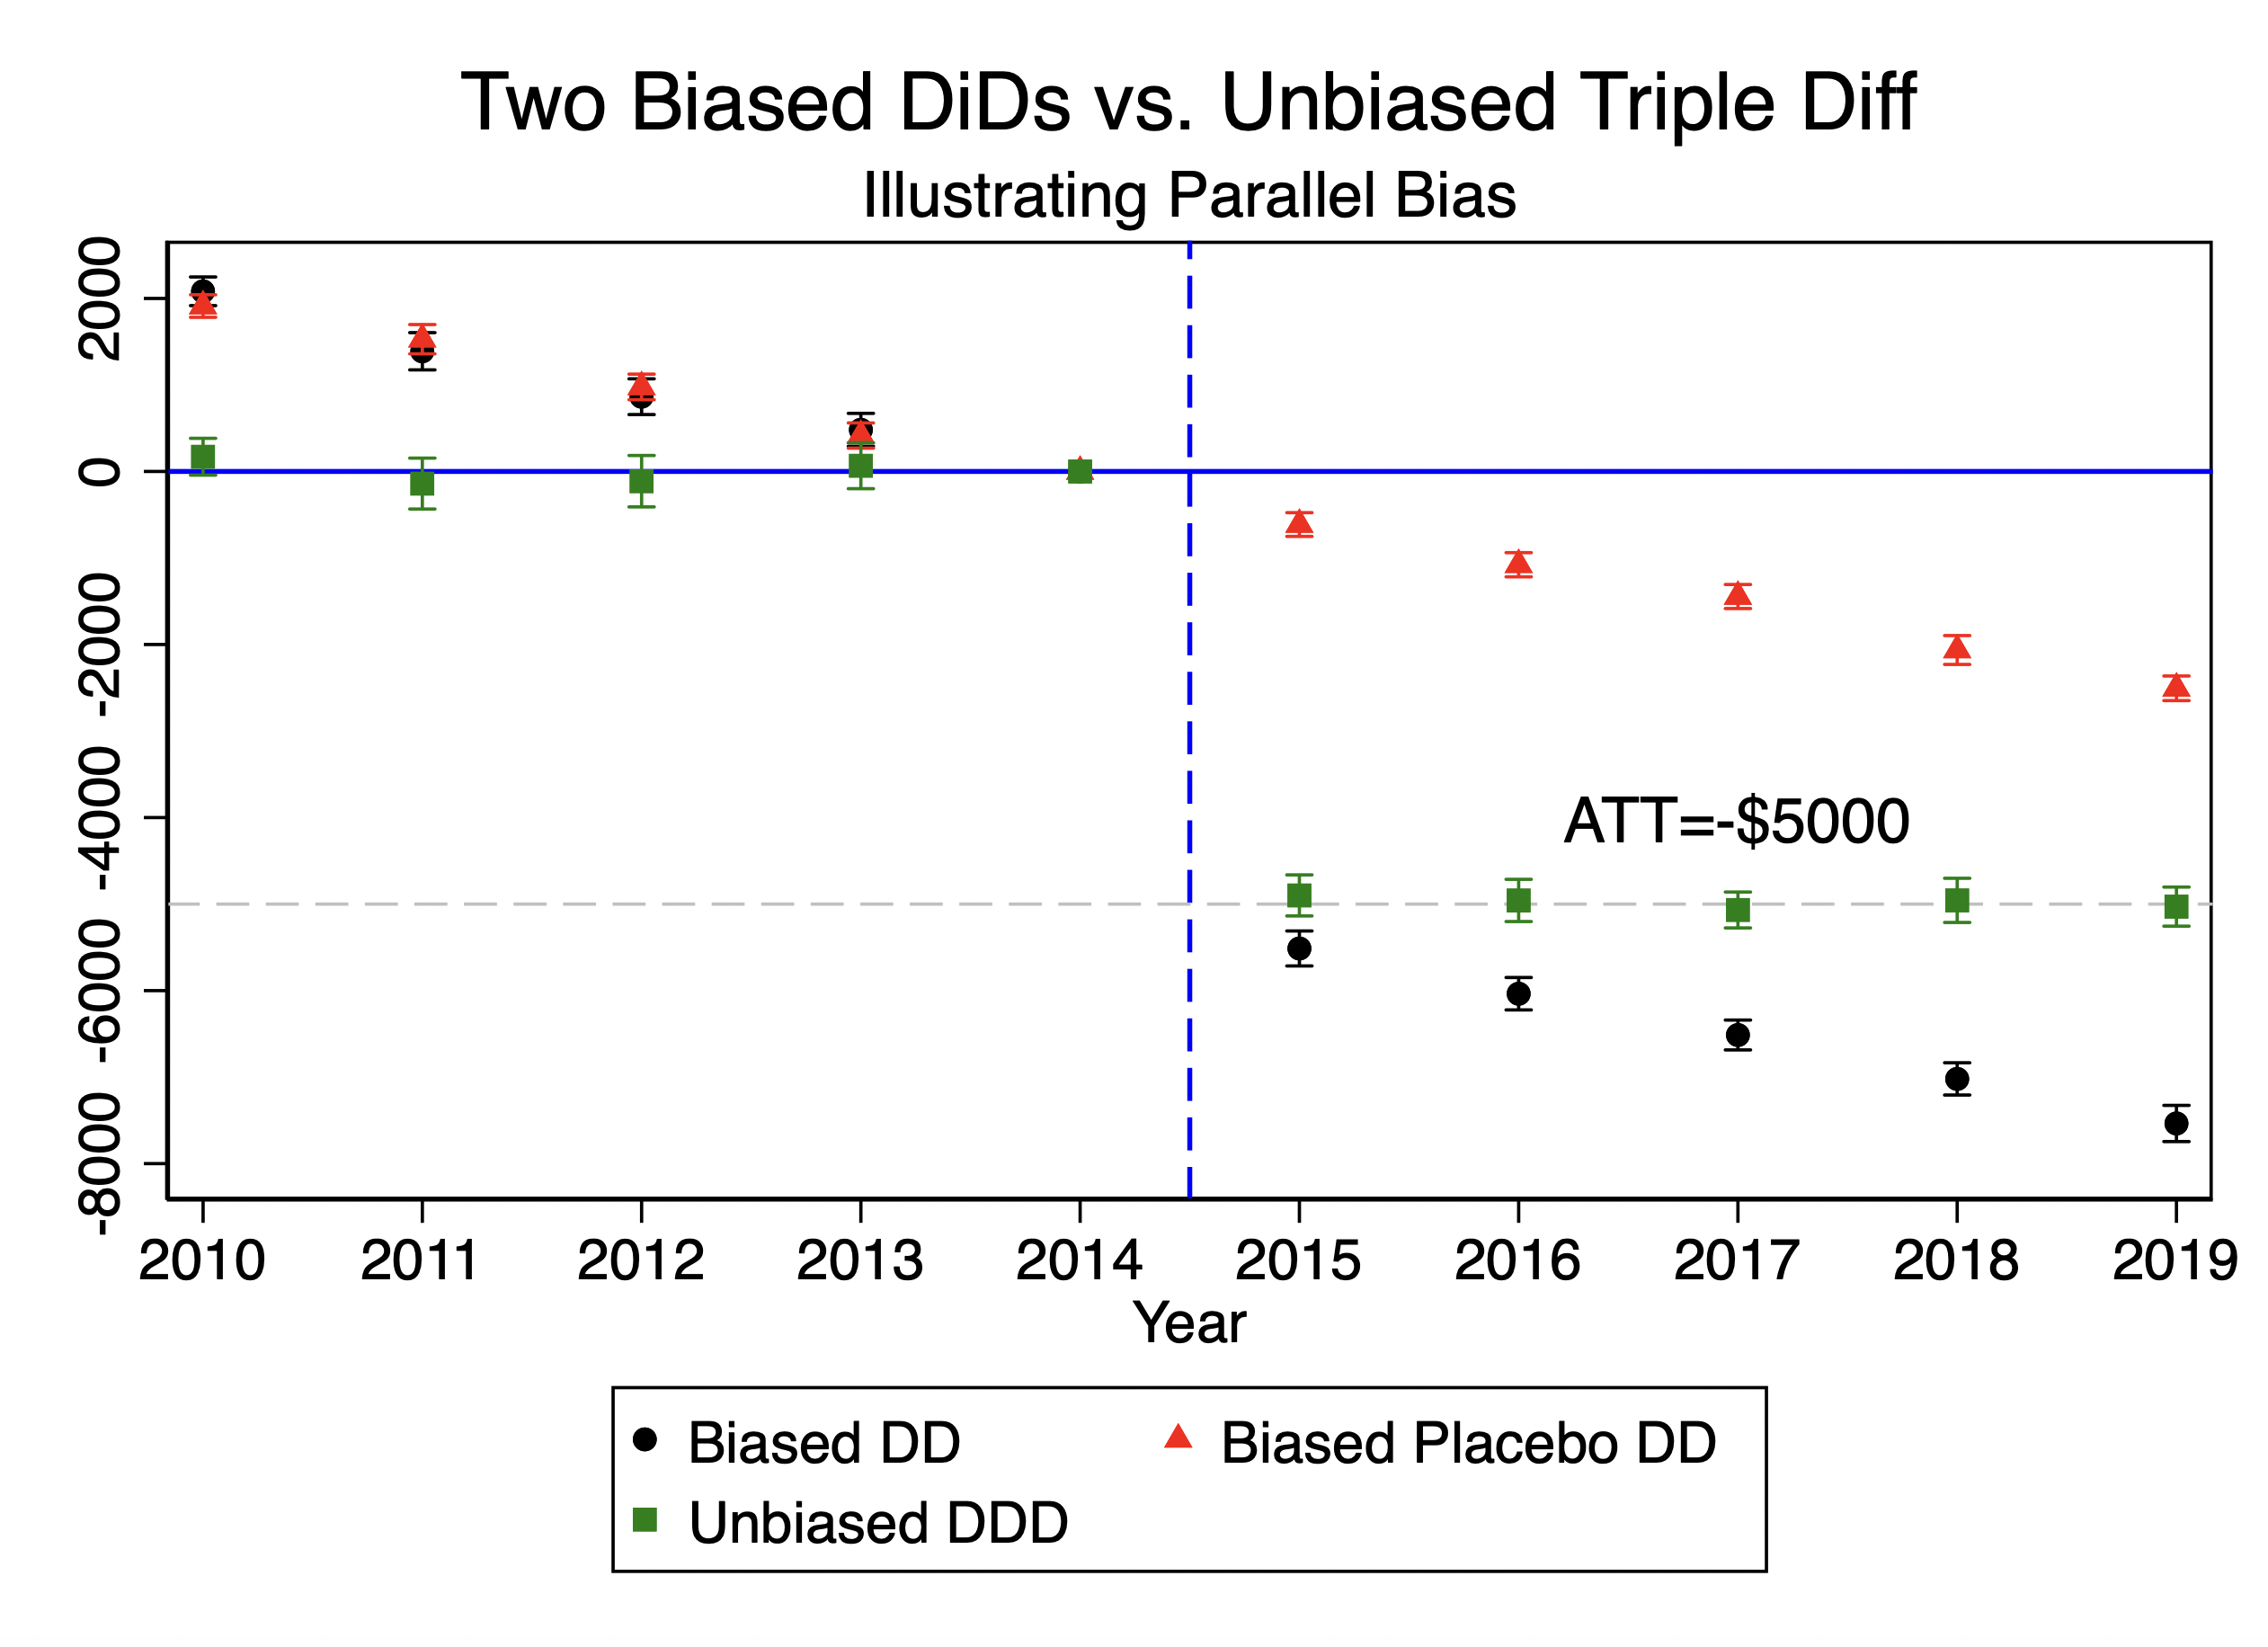
\includegraphics[scale=0.25]{./lecture_includes/ddd_simulation}
\end{figure}



\end{frame}  

\begin{frame}{Great new paper to learn more}

\begin{figure}
\includegraphics[scale=0.25]{./lecture_includes/olden_moen_2022_ddd.png}
\end{figure}

\end{frame}


\begin{frame}{Summarizing DDD}

\begin{itemize}
\item Used to be people thought DDD required two parallel trends assumptions but it does not -- it is a real design and requires one parallel trends assumption
\item Parallel trends assumption is ``parallel bias'' -- that the bias of the true DiD is the same as the bias of the placebo DiD
\item The ladder of evidence still holds -- you'll want to present the event study plot, and my code provides it for you, because you need to evaluate the parallel bias assumption
\item Given the lack of triple diff literacy, you may have to write this anticipating reader and maybe editor confusion and so "educate" as you go -- overlaying all three plots could be help

\end{itemize}

\end{frame}


\subsection{Falsifications}

\begin{frame}{Falsification on outcomes}
	
	\begin{itemize}
	\item Miller, Johnson and Wherry (2021) used the same outcome, but a placebo untreated treatment group (elderly) as a falsification to provide evidence for parallel trends
	\item But you can also use the same group but different outcomes
	\item Cheng and Hoekstra (2013) examine the effect of castle doctrine gun laws on non-gun related offenses like grand theft auto and find no evidence of an effect 
	\item You just want to pick things that make logical sense in that they are a similar enough group (near elderly versus elderly) or an outcome that would be susceptible to some omitted variable you're worried about
	\end{itemize}
\end{frame}



\begin{frame}{Rational addiction as a placebo critique}


Sometimes, an empirical literature may be criticized using nothing more than placebo analysis

\begin{quote}``A majority of [our] respondents believe the literature is a success story that demonstrates the power of economic reasoning.  At the same time, they also believe the empirical evidence is weak, and they disagree both on the type of evidence that would validate the theory and the policy implications. Taken together, this points to an interesting gap.  On the one hand, most of the respondents claim that the theory has valuable real world implications.  On the other hand, they do not believe the theory has received empirical support.''
\end{quote}

\end{frame}

\begin{frame}{Placebo as critique of empirical rational addiction}

\begin{itemize}
	\item Auld and Grootendorst (2004) estimated standard ``rational addiction'' models (Becker and Murphy 1988) on data with milk, eggs, oranges and apples.  
	\item They find these plausibly non-addictive goods are addictive, which casts doubt on the empirical rational addiction models.
\end{itemize}

\end{frame}

\begin{frame}{Placebo as critique of peer effects}

\begin{itemize}
	\item Several studies found evidence for ``peer effects'' involving inter-peer transmission of smoking, alcohol use and happiness tendencies
	\item Christakis and Fowler (2007) found significant network effects on outcomes like obesity
	\item Cohen-Cole and Fletcher (2008) use similar models and data and find similar network ``effects'' for things that \emph{aren't} contagious like acne, height and headaches
	\item Homophily (sorting) is probably just as likely an explanation
\end{itemize}

\end{frame}

\begin{frame}{Concluding the basics}


\begin{itemize}

\item That concludes the basics of diff-in-diff
\item A lot of what we just went through is pretty standard and common to any diff-in-diff, but some of it even other studies too
\item Notice how we really didn't address any parallel trends violation issues with much more than just looking for evidence that it probably held
\item But what if actually doesn't hold and we can't fix it with triple differences?  
\item Next we look at one very common example -- the use of covariates to fix parallel trends violations

\end{itemize}

\end{frame}


\end{document}


